\documentclass[a4paper,12pt,reqno]{article}
\usepackage{styledoc19}

\addbibresource{references.bib}

\begin{document}

\docNumber{RU.17701729.04.01-01 34 01-1}
\docFormat{Руководство оператора}
\student{БПИ 213}{В. А. Андронов}

\project{Веб-приложение для ведения лабораторных и вычислительных экспериментов с поддержкой онтологий\unskip}

\supervisor{Доцент департамента \vfill программной инженерии \vfill факультета компьютерных \vfill наук, кандидат \vfill технических наук}{О. В. Максименкова}

\firstPage
\newpage
\secondPage
\newpage
\thirdPage
\newpage

\section{Назначение программы}
\subsection{Функциональное назначение}
Разрабатываемое решение предоставляет возможность создавать, описывать, просматривать, редактировать и экспортировать эксперименты лабораторных и вычислительных экспериментов. Эксперименты описываются с привязкой к онтологиям из расширяемого набора возможных онтологий предметной области.

\subsection{Эксплуатационное назначение}
Приложение может использоваться в научных учреждениях, занимающихся в первую очередь химией и материаловедением, хотя возможна доработка для любой области, в которой уместно понятие эксперимента и для которой существуют подходящие онтологии. Конечными пользователями являются группы научных сотрудников, студенты, а также ML-разработчики и аналитики данных.

\subsection{Область применения}
Онтологически-контролируемое управление данными представляет собой современный подход к систематизации и обработке информации в химии и материаловедении. Данный метод основывается на использовании онтологий — формальных описаний концепций и их взаимосвязей в конкретной предметной области, что позволяет создать единое семантическое пространство для обмена знаниями и данными~\cite{ontology:base}.

В условиях увеличивающихся объемов данных и сложных междисциплинарных исследований, необходимость в эффективных инструментах управления информацией становится все более очевидной. Онтологически-контролируемое управление данными позволяет не только организовывать большие объемы информации, но и обеспечивать их интероперабельность. Это упрощает процессы интеграции данных из различных источников и способствует более тесному сотрудничеству между научными коллективами и организациями, занимающимися исследованиями в смежных областях.

\subsection{Состав выполняемых функций}

\subsubsection{Серверная часть}
Серверная часть приложения реализована с использованием фреймворков FastAPI~\cite{Framework:FastAPI} и SQLAlchemy~\cite{Library:SQLAlchemy}. Она отвечает за обработку запросов от клиента, управление данными о лабораторных и вычислительных экспериментах, а также интеграцию с онтологиями. Серверная часть включает в себя:
\begin{itemize}
    \item Обработку API-запросов для работы с экспериментами (создание, редактирование, удаление, получение данных).
    \item Аутентификацию и авторизацию пользователей с использованием JWT~\cite{Security:JWT}.
    \item Работа с реляционной базой данных для хранения информации о пользователях, экспериментах, измерениях и онтологиях.
    \item Интеграцию с графовой базой данных для работы с онтологиями.
\end{itemize}

\subsubsection{Клиентская часть}
Клиентская часть приложения реализована на Vue.js~\cite{Framework:VueJS} с использованием PrimeVue~\cite{Framework:PrimeVue} для UI-компонентов. Она предоставляет пользователю удобный интерфейс для взаимодействия с системой, включая:
\begin{itemize}
    \item Вход и регистрация для пользователей.
    \item Страницы управления экспериментами и шаблонами вычислительных экспериментов (создание, редактирование, просмотр, удаление).
    \item Интеграцию с сервером через REST API для работы с данными о лабораторных и вычислительных экспериментах.
    \item Страницу работы с онтологиями, где пользователи могут привязывать исследовать содержимое доступных онтологий.
    \item Поддержку адаптивного дизайна для работы на различных устройствах.
\end{itemize}

\section{Условия выполнения программы}

\subsection{Минимальный состав аппаратурных средств}

Для надежной и бесперебойной работы программы требуется следующий состав аппаратурных средств:

\begin{enumerate}
    \item Компьютер, оснащенный процессором Intel Core i5 с тактовой частотой 2,3 ГГц;
    \item 16 Гб ОЗУ;
    \item Жесткий диск с объемом свободной памяти более чем 50 ГБ;
    \item Клавиатура и мышь;
    \item Доступ в интернет.
\end{enumerate}

\subsection{Минимальный состав программных средств}

Для надежной и бесперебойной работы программы требуется следующий состав программных средств:
\begin{enumerate}
    \item macOS 10.15.4 или Windows 10 
    \item Google Chrome;
    \item Docker.
\end{enumerate}

\subsection{Требования к пользователю}

Пользователь должен быть ознакомлен с терминологией, представленной в Приложении~\ref{additionterms}. Также пользователь должен быть знаком на базовом уровне с аппаратурными средствами.

\section{Выполнение программы}

\subsection{Загрузка и запуск программы}

\subsubsection{Заполнение конфигурации}

Для запуска приложения нужно клонировать репозиторий, перейти в корень проекта. Перед запуском потребуется создать или отредактировать файлы переменных окружения для всех компонентов. Для этого используются файлы \texttt{.env} в корне проекта и в директории \texttt{backend/config}.В них указываются параметры подключения к базам данных, секретные ключи, настройки портов и прочие параметры. Пример содержимого файла \texttt{.env} в листинге~\ref{lst:config_all}.
\begin{lstlisting}[frame=single, basicstyle=\footnotesize\ttfamily, label={lst:config_all}, caption={Заполнение конфигурационного файла всего приложения},captionpos=b, breaklines=true, breakatwhitespace=true, language=bash]
PG_USER=postgres
PG_PASSWORD=123
PG_DB=postgres

NEO4J_USER=neo4j
NEO4J_PASSWORD=123
\end{lstlisting}

Для запуска серверного приложения требуется создание в директории \texttt{backend/config} файла \texttt{config.stable.toml}, в котором нужно в формате TOML~\cite{Format:TOML} определить по крайней мере параметры \texttt{db.host}, \texttt{db.password}, \texttt{neo4j.host}, \texttt{neo4j.password}.
Также необходимо зарегистрировать онтологии по следующему принципу: секция \texttt{ontologies} представляет собой отображение, где ключ являются псевдонимом онтологий, которое затем может быть использовано в клиентском приложении, а значением – название метки, которая должна быть у каждого элемента онтологии.
Таким образом, если есть в секции \texttt{ontologies} пара, например, (OM2, om2UniqueLabel) приложение будет интерпретировать всякий результат запроса в Neo4j с меткой om2UniqueLabel как элемент онтологии OM2.

Пример содержимого файла \texttt{backend/config/config.stable.toml} в листинге~\ref{lst:config_backend}.
\begin{lstlisting}[frame=single, basicstyle=\footnotesize\ttfamily, label={lst:config_backend}, caption={Заполнение конфигурационного файла серверного приложения},captionpos=b, breaklines=true, breakatwhitespace=true]
[uvi]
host = ""
port = 0
workers = 0
timeout = 0
debug = false

[db]
port = 0
user = ""
database = ""
echo = false
echo_pool = false
pool_size = 0
max_overflow = 0
host = ""
password = ""

[neo4j]
port = 0
user = ""
db = ""
host = ""
password = ""

[jwt]
algorithm = ""
access_token_expire_minutes = 0
private_key_path = ""
public_key_path = ""
refresh_token_expire_minutes = 0

[ontologies]
OM2 = '__OntologyOM2__'
ChEBI = '__OntologyChEBI__'
\end{lstlisting}

\subsubsection{Запуск с помощью Docker Compose}

После настройки переменных окружения приложение запускается одной командой: \texttt{docker-compose up --build}.
Эта команда соберёт и запустит все необходимые сервисы: серверную часть, клиентскую часть, базы данных PostgreSQL и Neo4j, а также Nginx для проксирования запросов.

Для запуска в фоновом режиме можно использовать флаг \texttt{-d}: \texttt{docker-compose up --build -d}

\subsubsection{Дополнительные команды}

Для управления жизненным циклом приложения используются стандартные команды Docker Compose:
\begin{itemize}
    \item Остановить сервисы: \texttt{docker-compose down}
    \item Перезапустить сервисы: \texttt{docker-compose restart}
    \item Просмотреть логи: \texttt{docker-compose logs -f}
\end{itemize}

\subsubsection{Доступ к приложению}

После успешного запуска приложение становится доступно по адресу, указанному в настройках Nginx (по умолчанию \texttt{http://localhost/}).
Все компоненты приложения взаимодействуют друг с другом через внутреннюю сеть Docker Compose.

\subsection{Работа в интерфейсе пользователя}

\subsubsection{Экран: Онтология ChEBI}

На этом экране отображается список элементов онтологии ChEBI с их описанием и URI. Для того чтобы использовать компоненты на этом экране:
\begin{enumerate}
    \item Вы можете фильтровать элементы по названию с помощью поисковой строки в верхней части экрана.
    \item Каждая строка отображает название вещества, комментарий и URI ссылки на соответствующий элемент онтологии.
    \item С помощью URI можно перейти к более подробной информации о веществе на внешнем ресурсе.
\end{enumerate}
\begin{figure}[H]
    \centering
    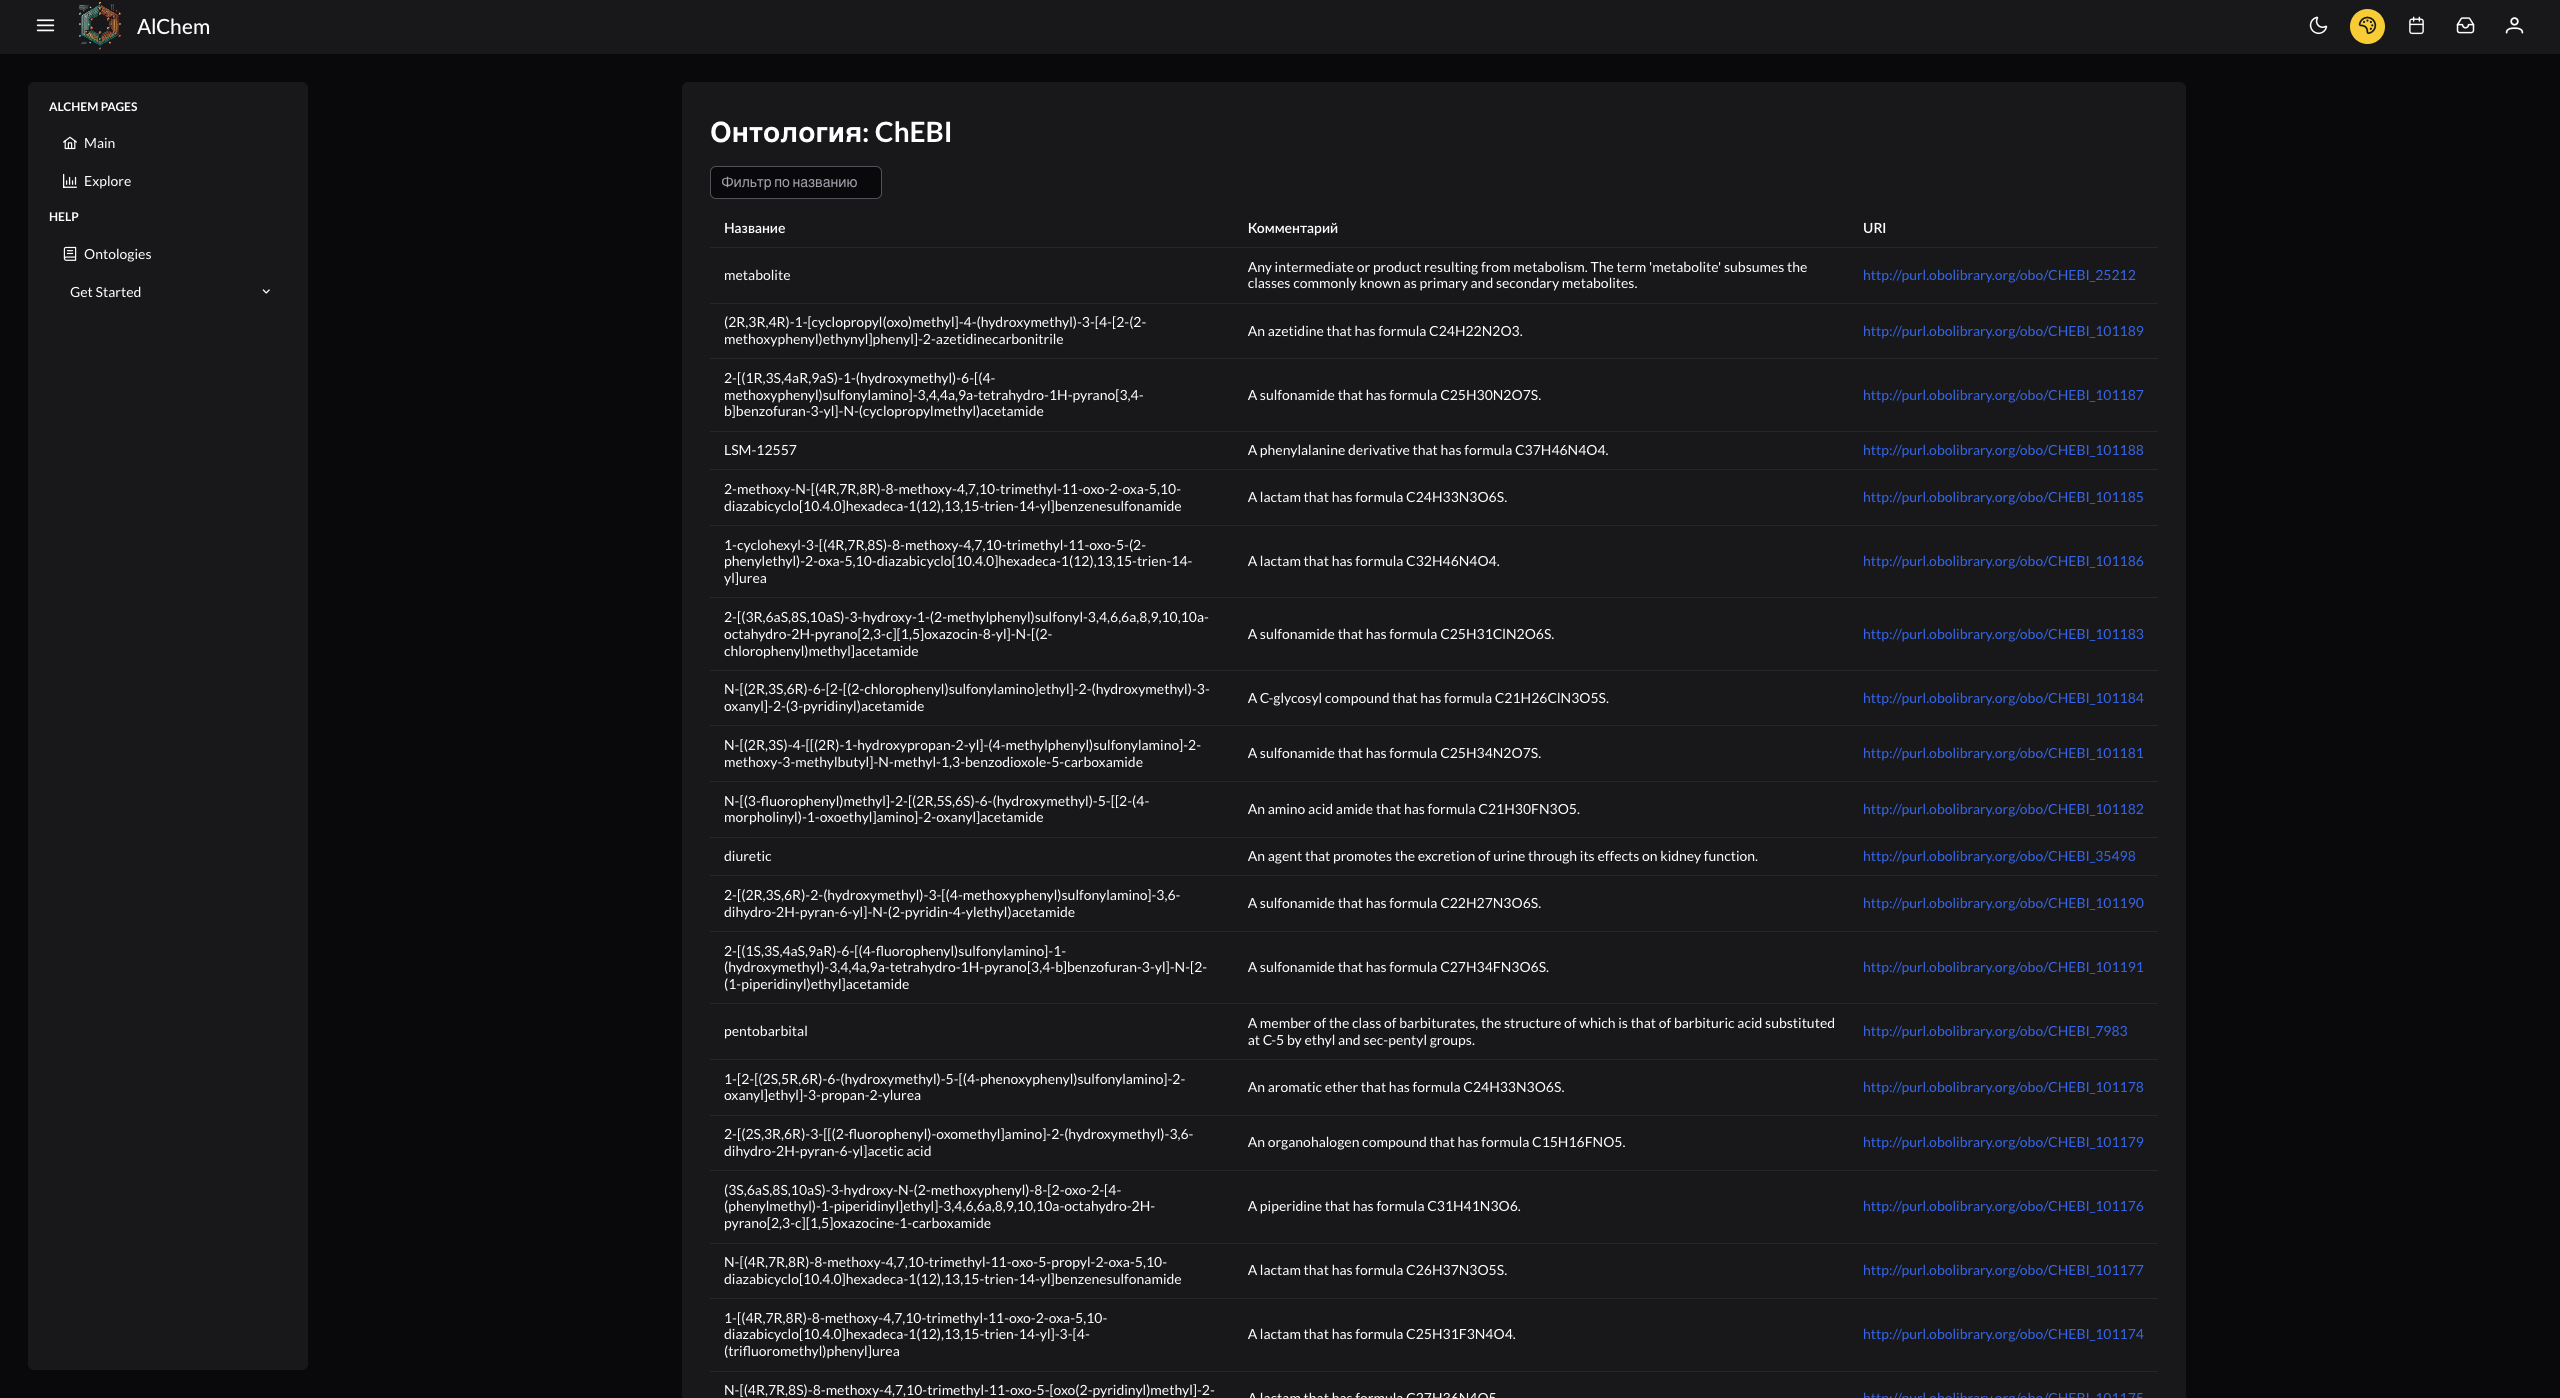
\includegraphics[width=\textwidth]{RO/img/chebi_doc.png} % Замените на правильный путь к изображению
    \caption{Экран: Онтология ChEBI}
    \label{fig:chebi}
\end{figure}

\subsubsection{Экран: Онтология OM2}

На этом экране представлен список единиц измерения, относящихся к измерениям физических величин, с их описанием и URI. Чтобы использовать этот экран:
\begin{enumerate}
    \item Фильтровать элементы по названию с помощью строки поиска.
    \item Каждый элемент включает в себя название единицы измерения, описание и ссылку на URI для получения дополнительных сведений.
    \item URI используется для перехода к более детализированной информации о единице измерения в системе OM2.
\end{enumerate}
\begin{figure}[H]
    \centering
    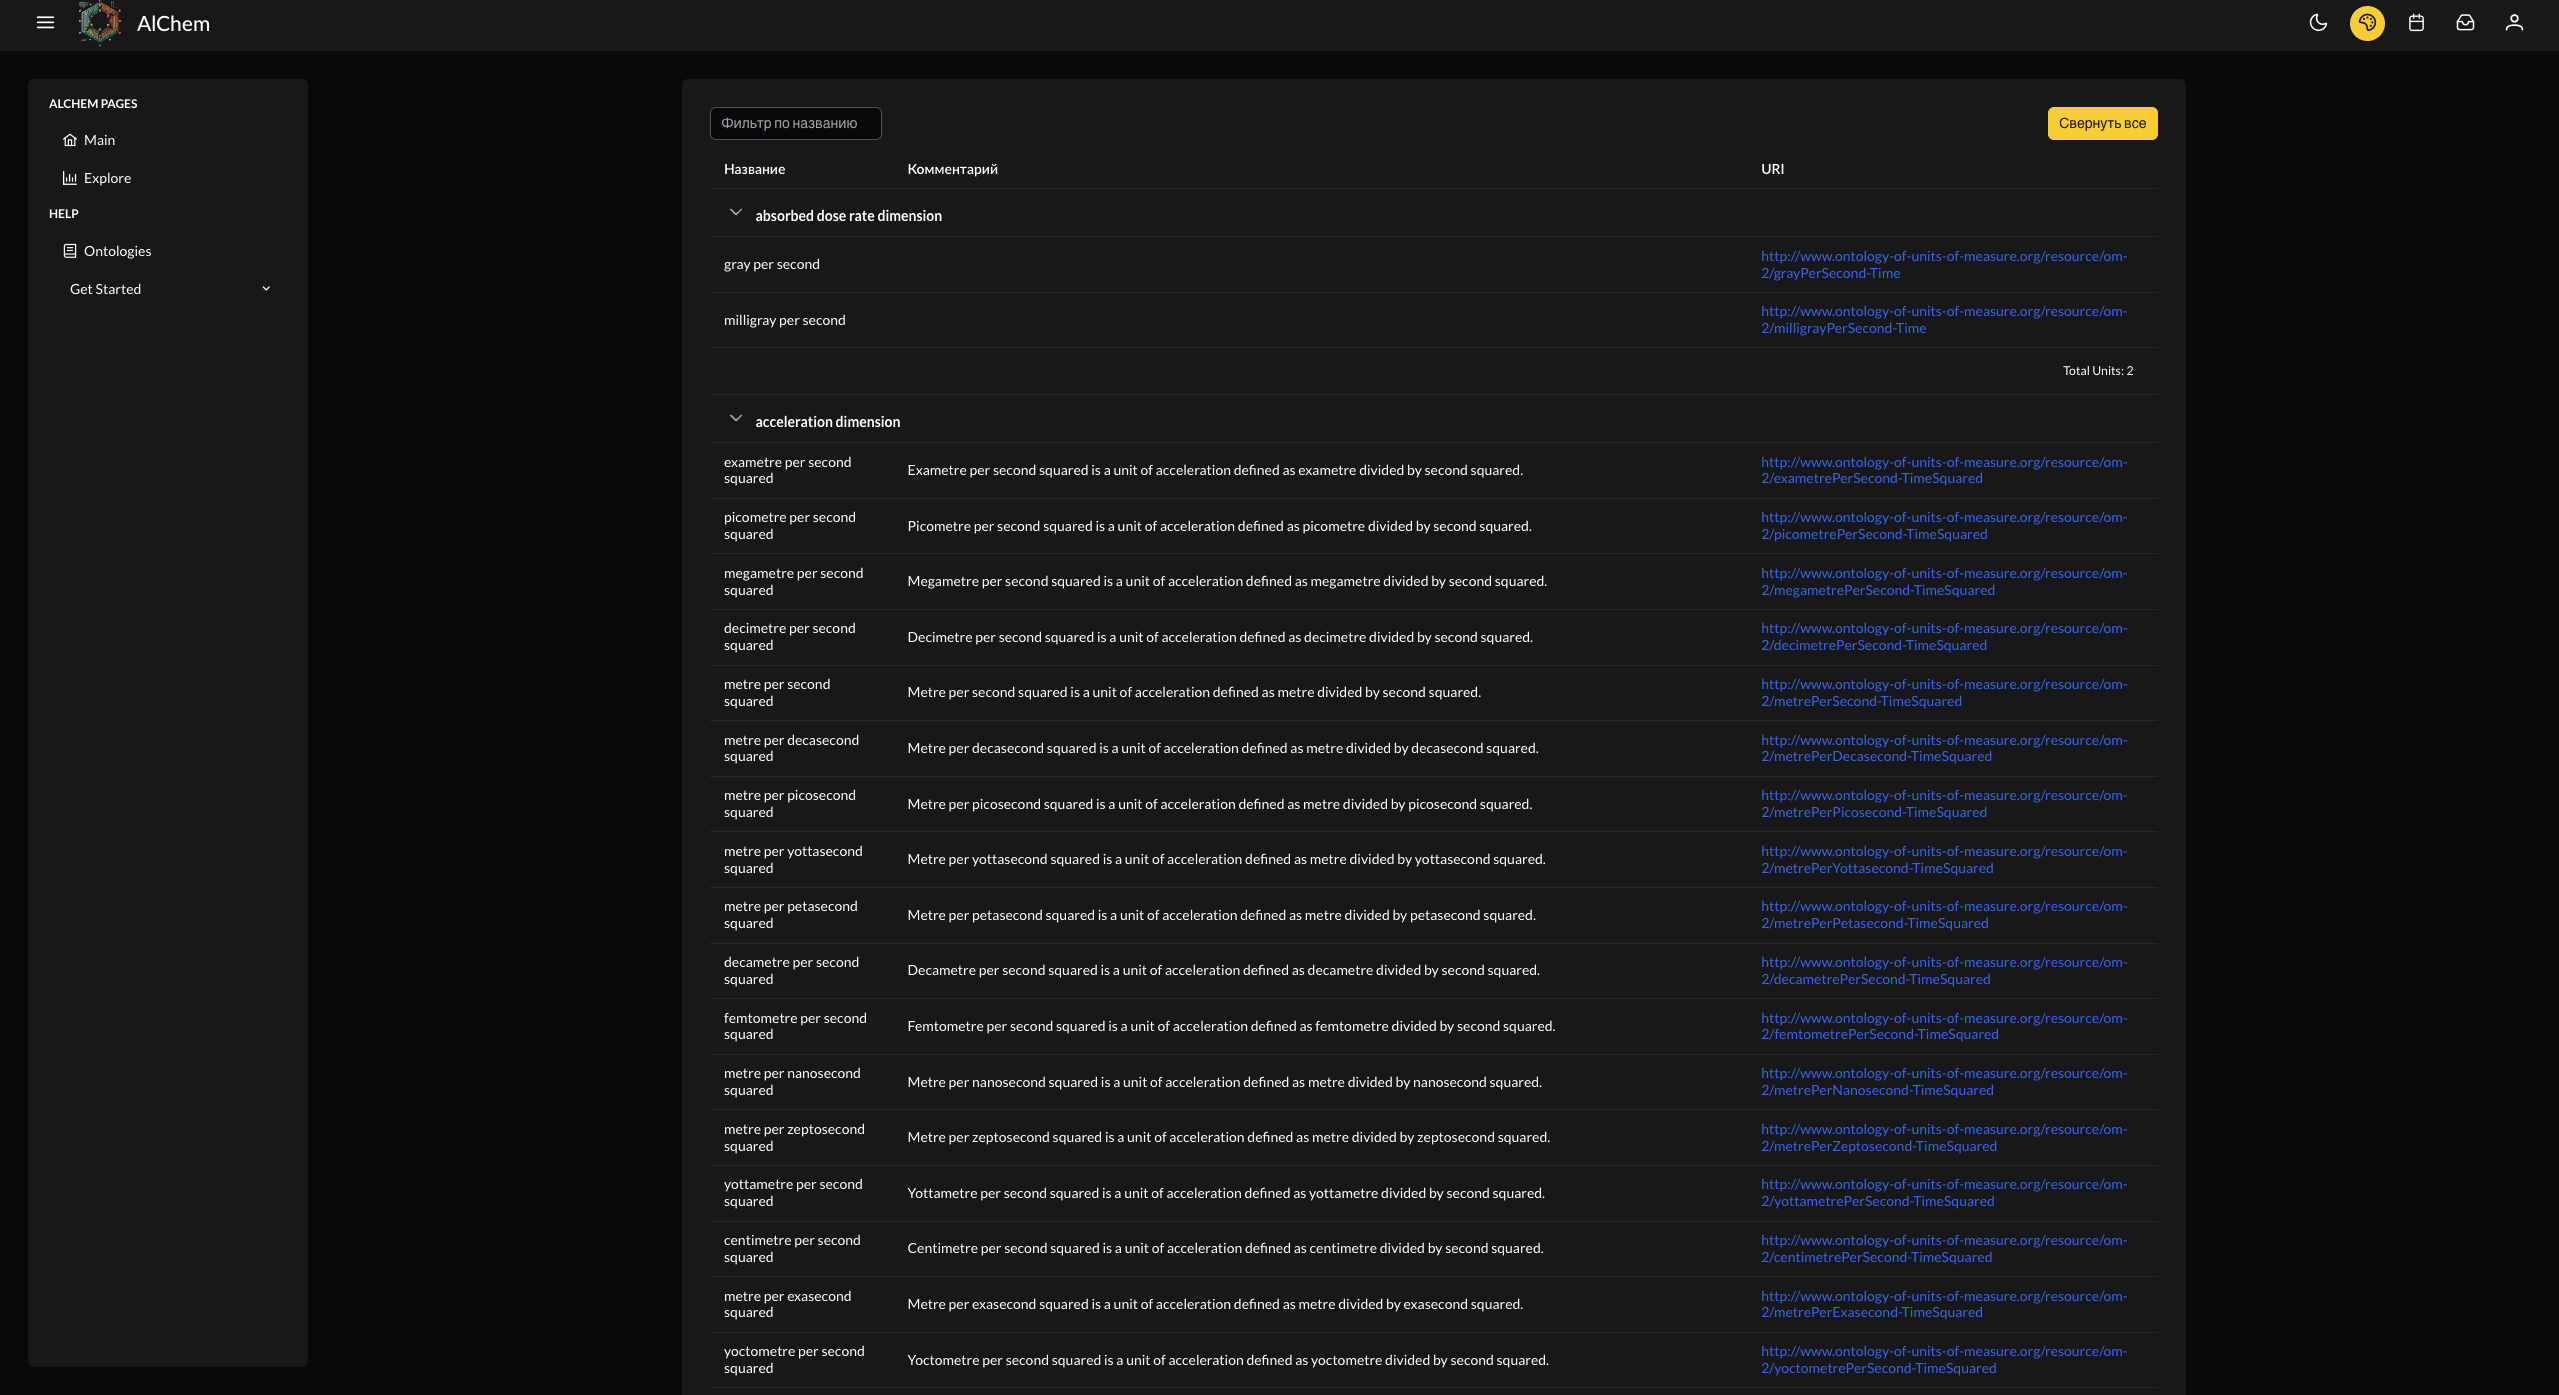
\includegraphics[width=\textwidth]{RO/img/om2_doc.png} % Замените на правильный путь к изображению
    \caption{Экран: Онтология OM2}
    \label{fig:om2}
\end{figure}

\subsubsection{Экран: Доступные онтологии}
На этом экране отображается список доступных онтологий:
\begin{enumerate}
    \item Выберите одну из доступных онтологий.
    \item После выбора онтологии вы сможете просматривать данные, связанные с ней, на специальных страницах приложения.
\end{enumerate}
\begin{figure}[H]
    \centering
    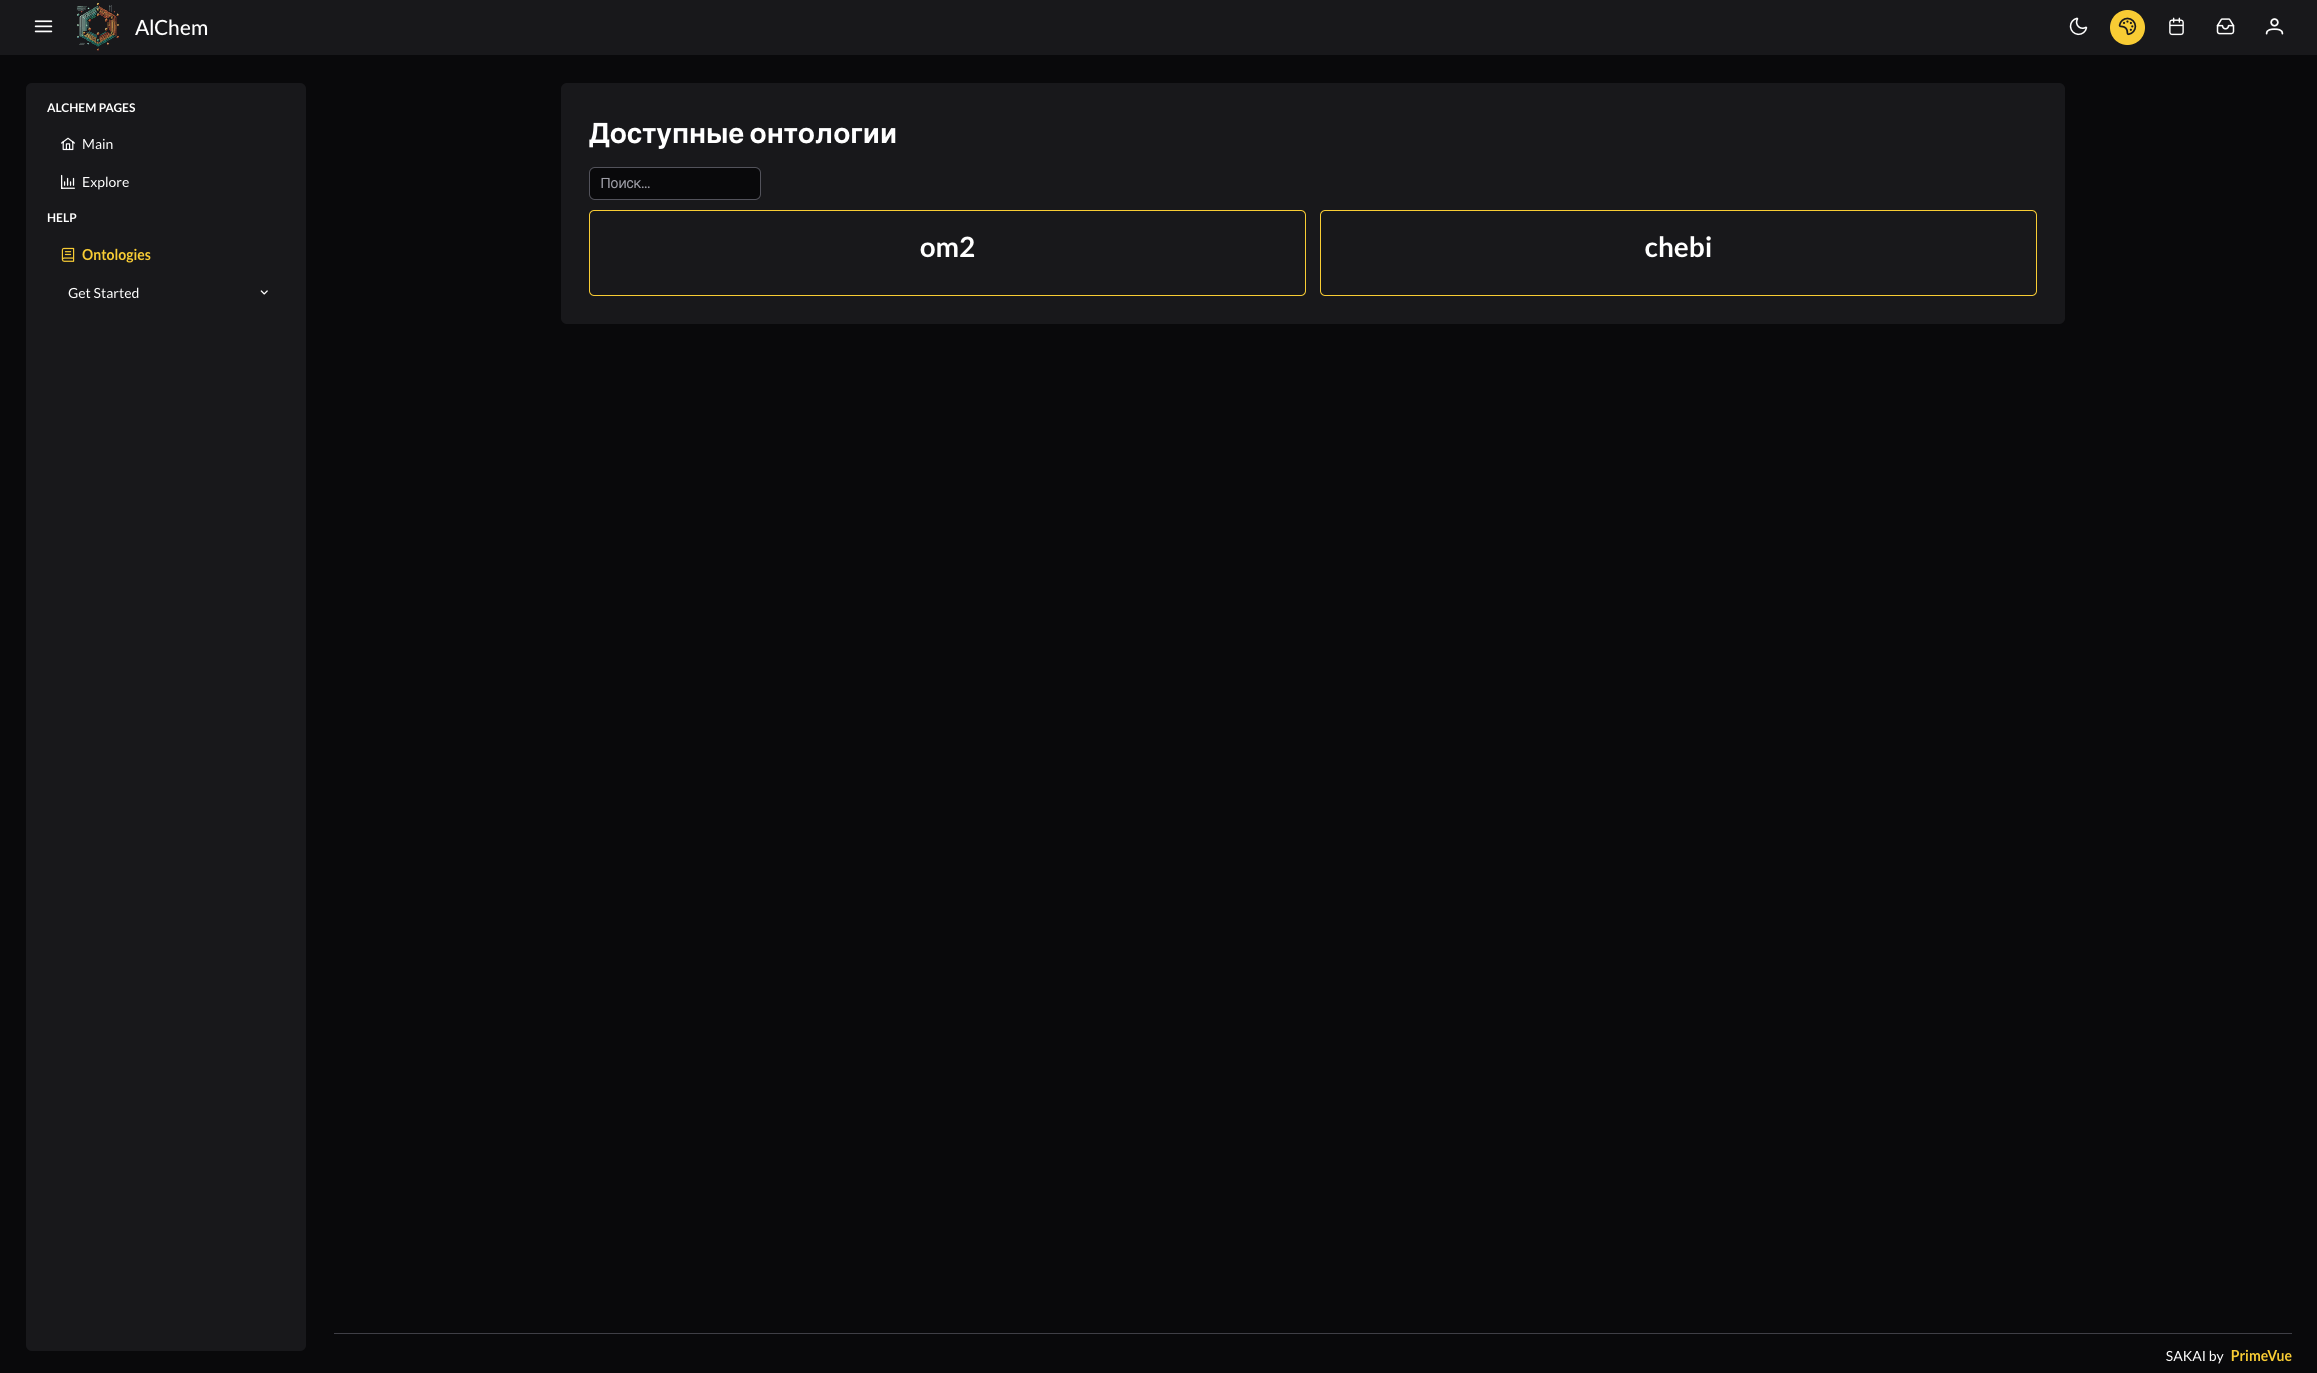
\includegraphics[width=\textwidth]{RO/img/common_doc.png} % Замените на правильный путь к изображению
    \caption{Экран: Доступные онтологии}
    \label{fig:common}
\end{figure}

\subsubsection{Экран: Сравнение экспериментов}
\textbf{Данные для ввода:}  
На этом экране отображается графическое сравнение двух экспериментов по заданным параметрам:
\begin{enumerate}
    \item Выберите несколько экспериментов из списка.
    \item Выберите один столбец для назначения его главным, например, температура.
    \item Выберите параметры для сравнения, например, длина и масса.
    \item Графики будут отображать зависимость главного столбца от параметров для всех выбранных экспериментов.
\end{enumerate}
\begin{figure}[H]
    \centering
    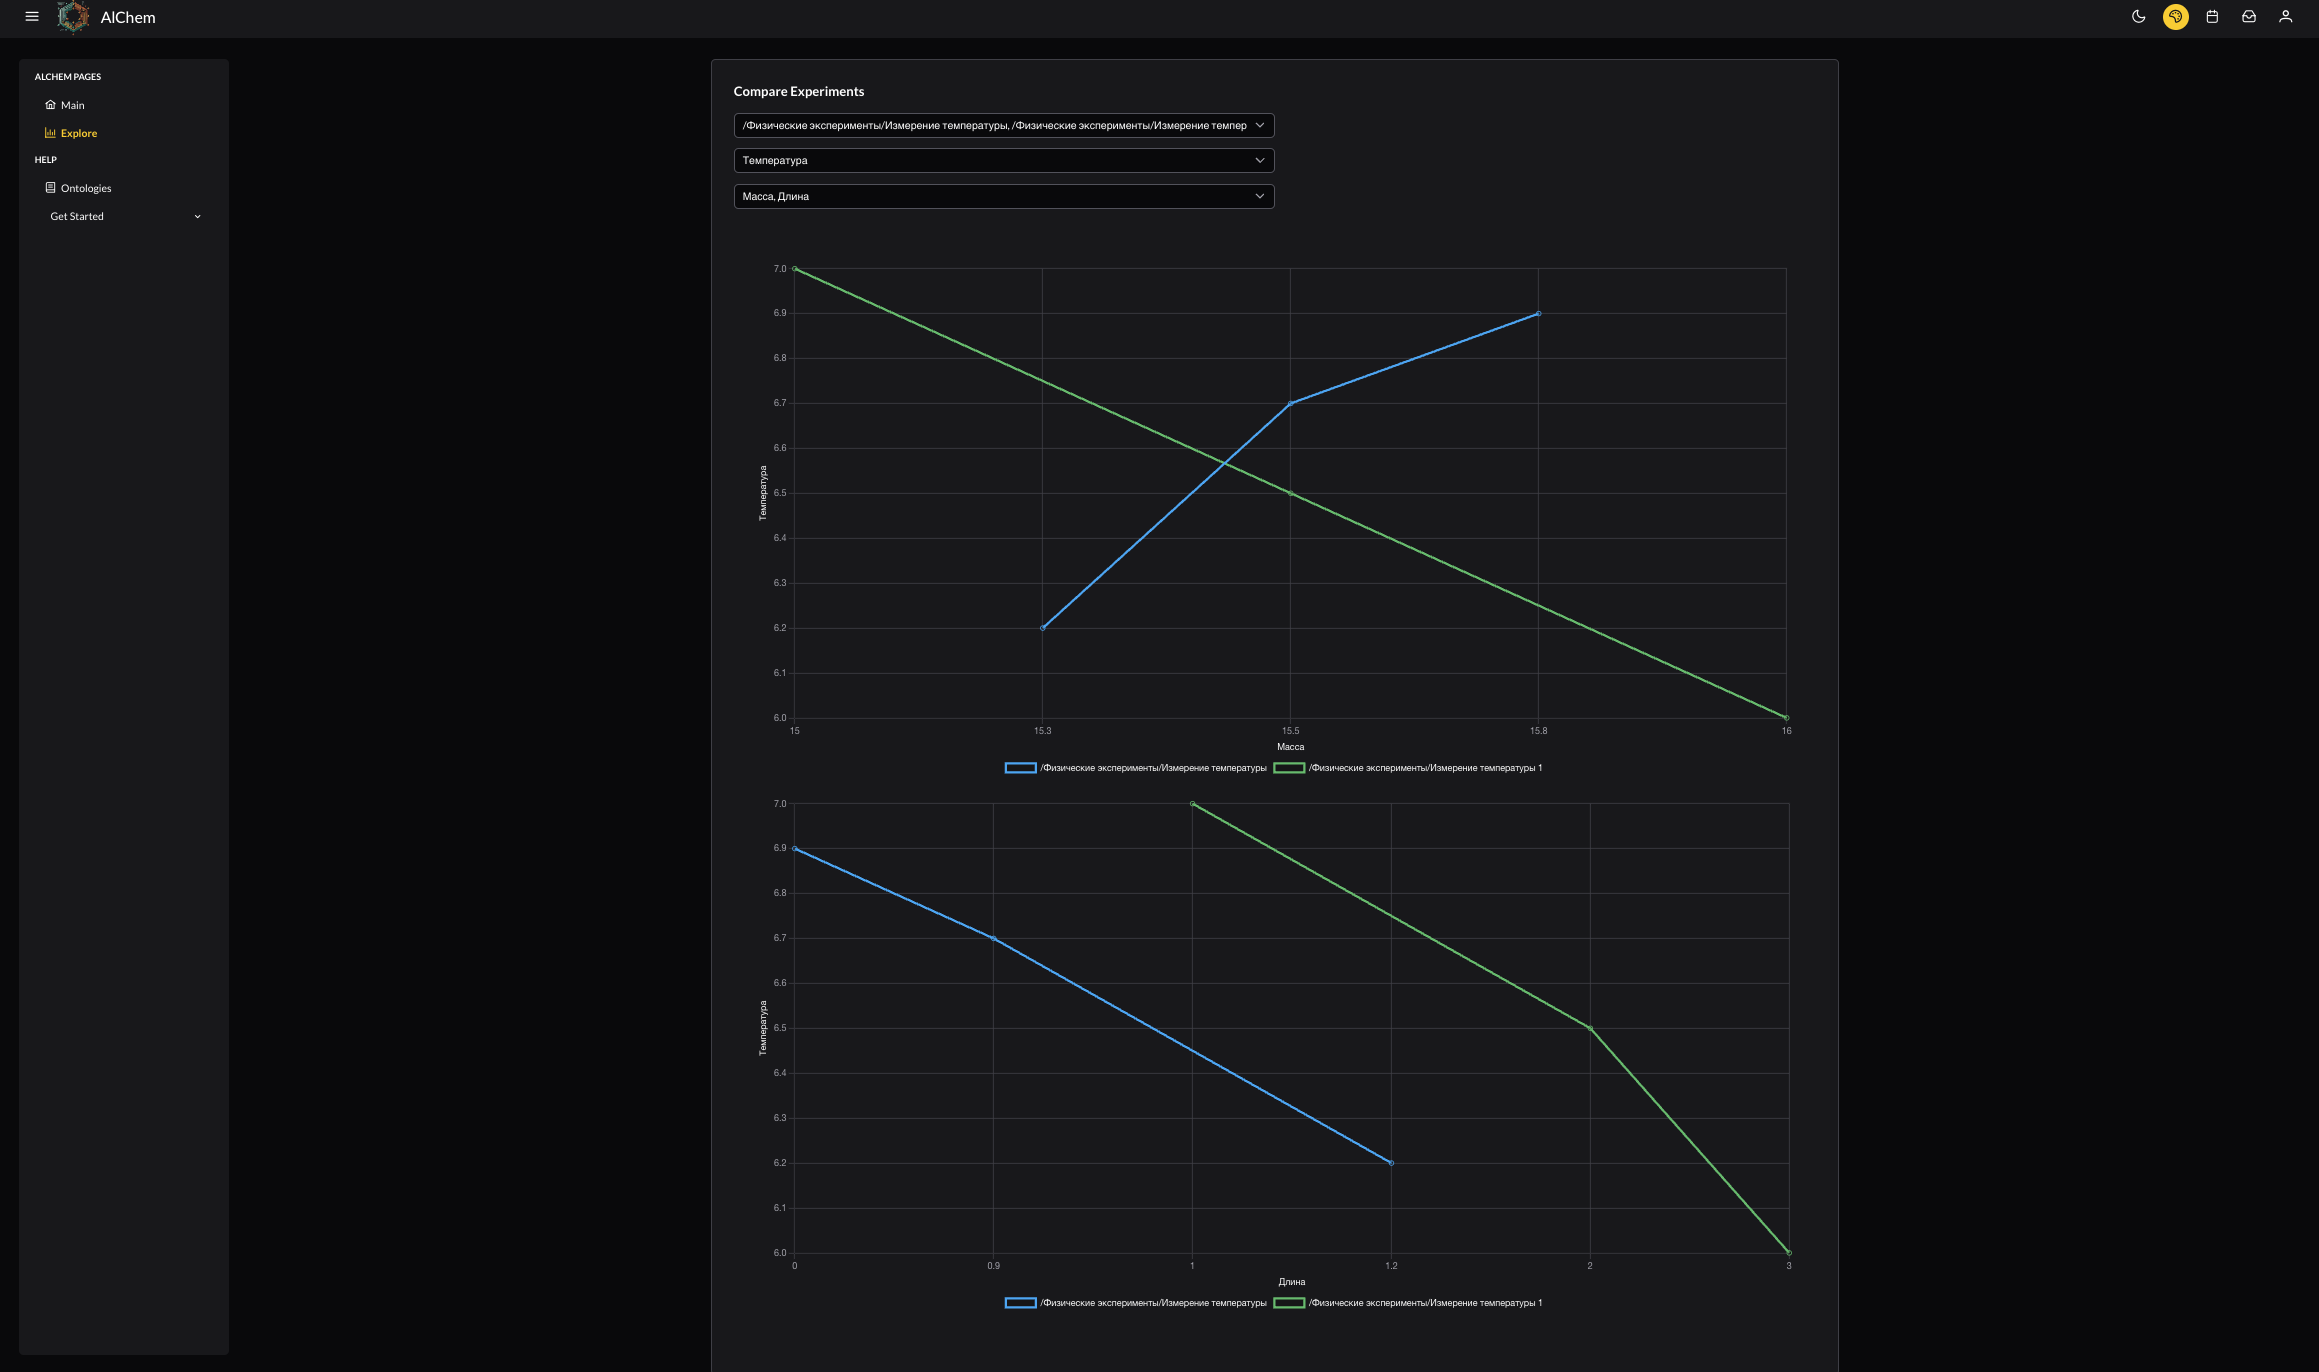
\includegraphics[width=\textwidth]{RO/img/multiple_doc.png} % Замените на правильный путь к изображению
    \caption{Экран: Сравнение экспериментов}
    \label{fig:compare_experiments}
\end{figure}

\subsubsection{Экран: Создание шаблона для вычислительного эксперимента}
\textbf{Данные для ввода:}
Для создания шаблона вычислительного эксперимента:
\begin{enumerate}
    \item Введите название шаблона.
    \item Укажите путь для хранения шаблона.
    \item Укажите схемы входных данных, выходных данных, параметров и контекста для шаблона.
    \item Нажмите "Создать" для сохранения шаблона.
\end{enumerate}
\begin{figure}[H]
    \centering
    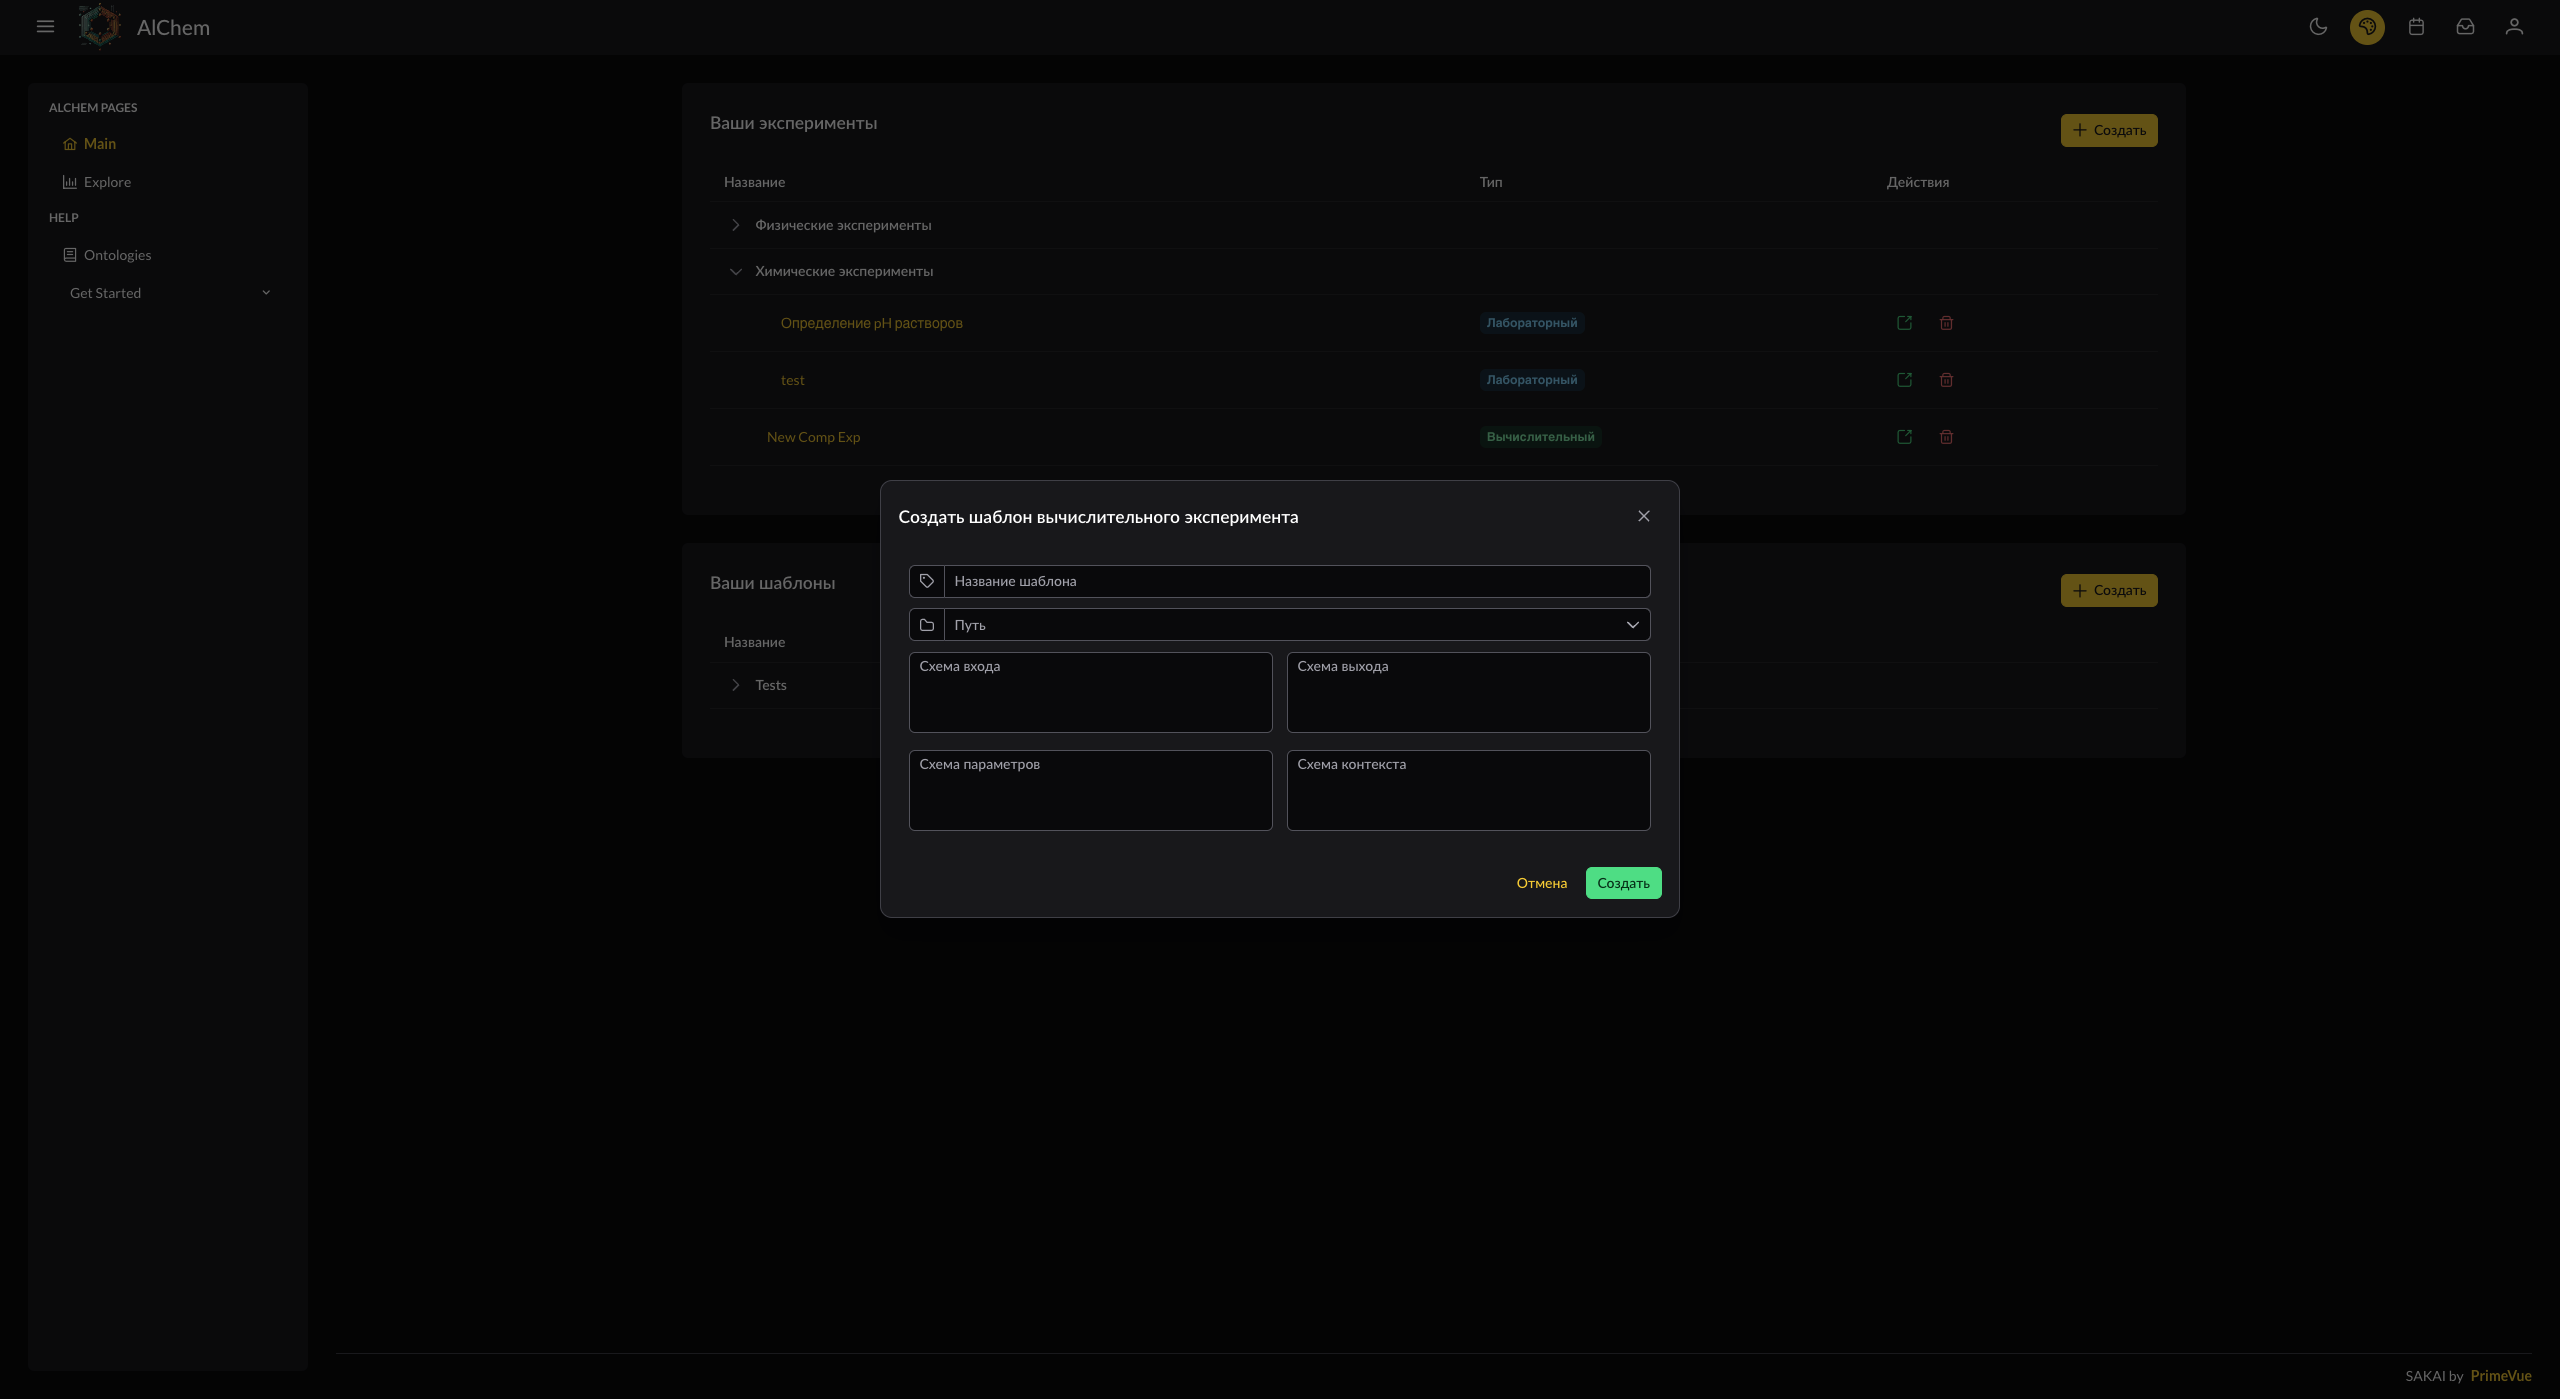
\includegraphics[width=\textwidth]{RO/img/create_template.png} % Замените на правильный путь к изображению
    \caption{Экран: Создание шаблона для вычислительного эксперимента}
    \label{fig:create_template}
\end{figure}

\subsubsection{Экран: Создание вычислительного эксперимента}
\textbf{Данные для ввода:} 
Для создания вычислительного эксперимента:
\begin{enumerate}
    \item Выберите тип эксперимента: вычислительный.
    \item Введите название эксперимента.
    \item Укажите путь, по которому будет сохранен эксперимент.
    \item Выберите шаблон для вычислительного эксперимента.
    \item Нажмите кнопку "Создать" для добавления нового эксперимента в систему.
\end{enumerate}
\begin{figure}[H]
    \centering
    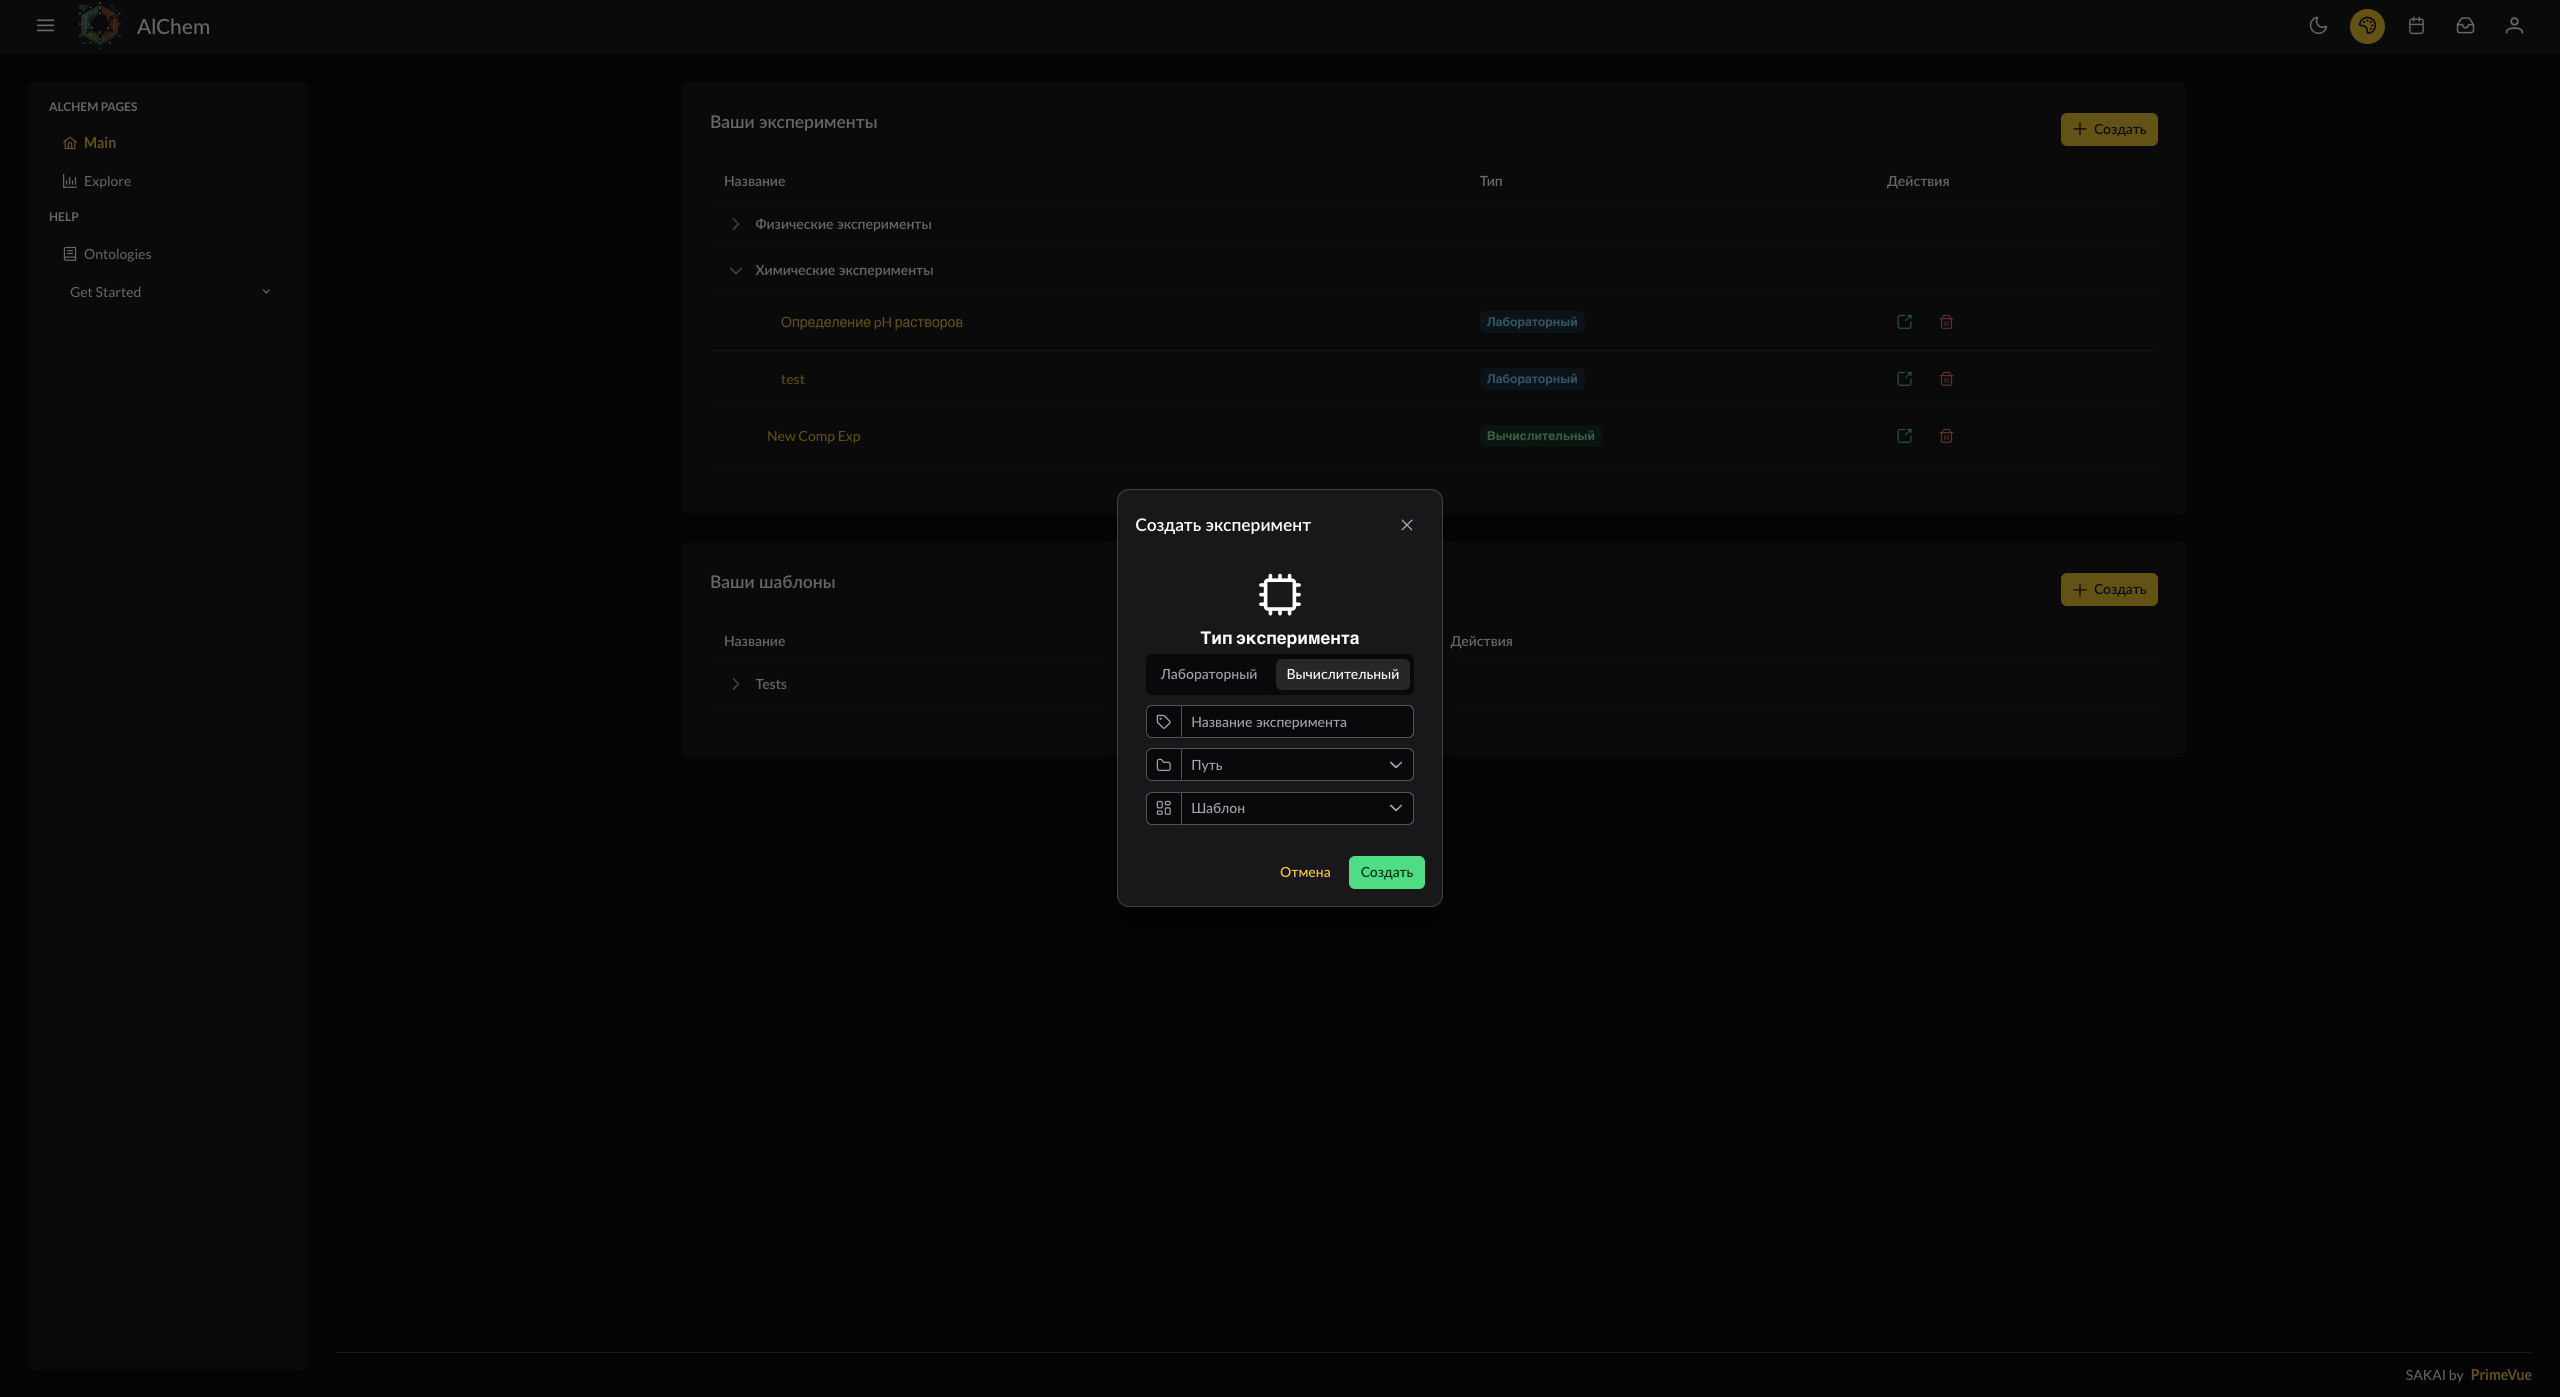
\includegraphics[width=\textwidth]{RO/img/create_exp.png} % Замените на правильный путь к изображению
    \caption{Экран: Создание вычислительного эксперимента}
    \label{fig:create_exp}
\end{figure}

\subsubsection{Экран: Создание лабораторного эксперимента}
\textbf{Данные для ввода:}  
Для создания лабораторного эксперимента:
\begin{enumerate}
    \item Выберите тип эксперимента: лабораторный.
    \item Укажите название эксперимента.
    \item Укажите путь, по которому будет сохранен эксперимент.
    \item Нажмите кнопку "Создать" для добавления эксперимента в систему.
\end{enumerate}
\begin{figure}[H]
    \centering
    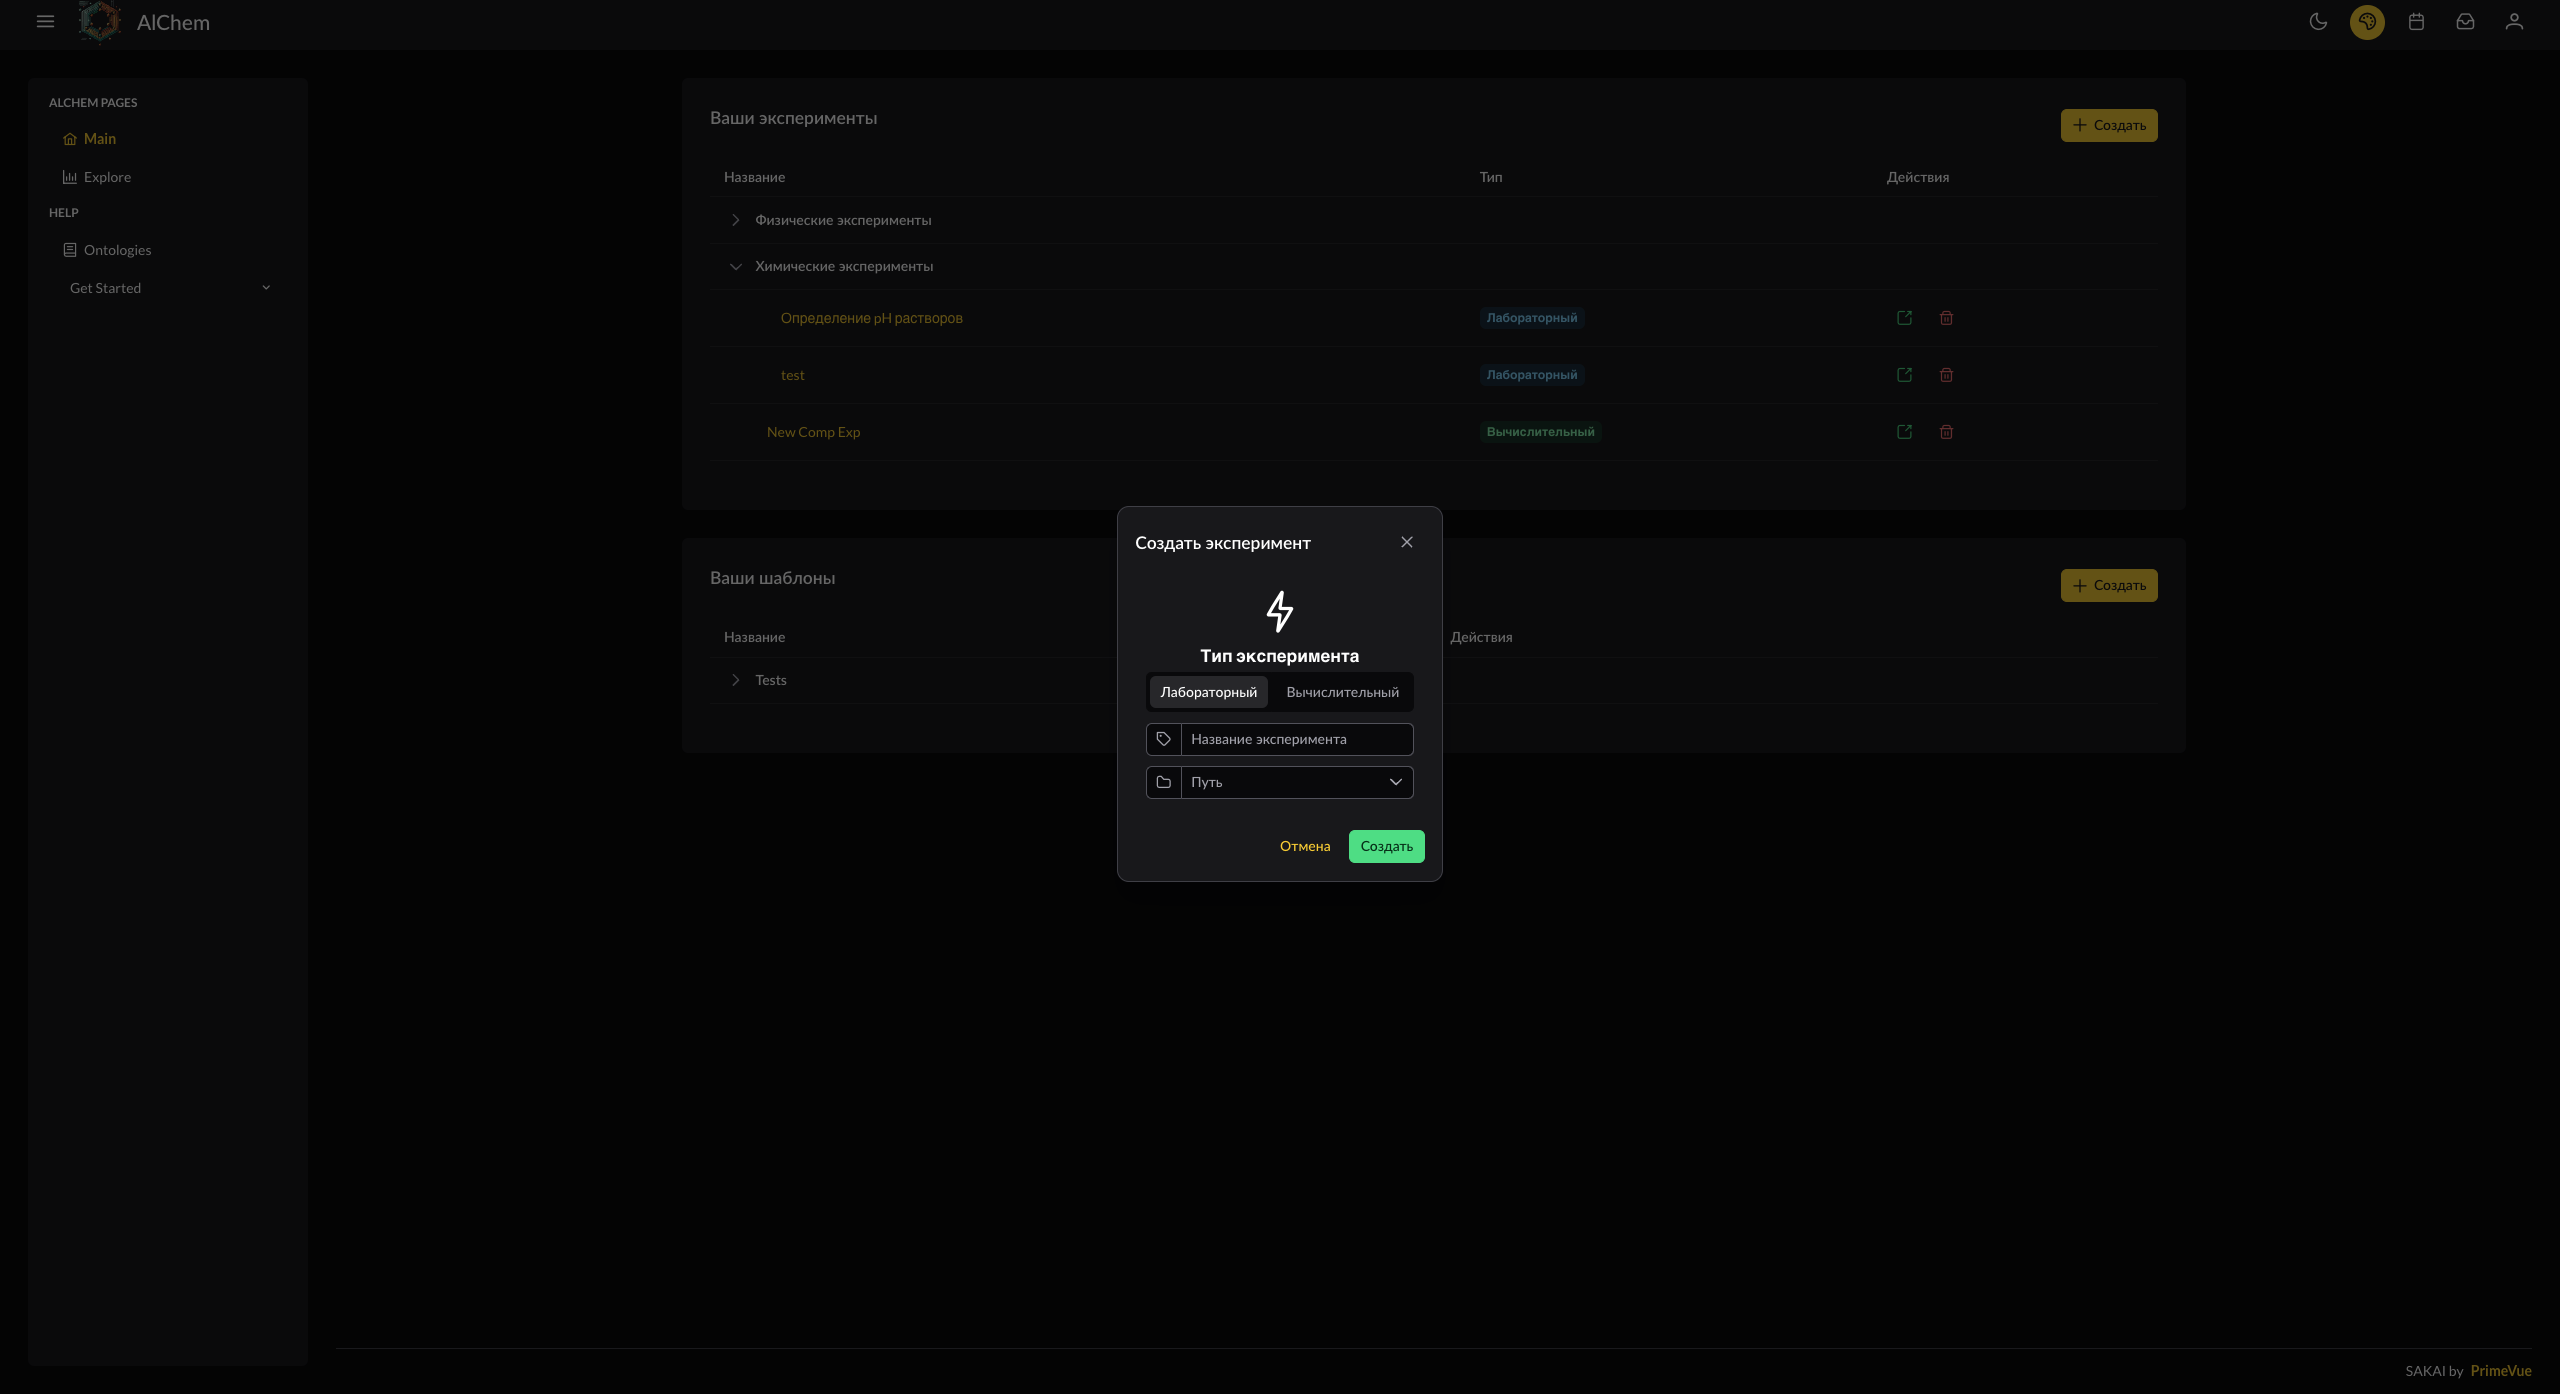
\includegraphics[width=\textwidth]{RO/img/create_lab.png} % Замените на правильный путь к изображению
    \caption{Экран: Создание лабораторного эксперимента}
    \label{fig:create_lab}
\end{figure}

\subsubsection{Экран: Создание папки}
\textbf{Данные для ввода:}  
Для создания новой папки для экспериментов:
\begin{enumerate}
    \item Укажите название папки.
    \item Выберите родительскую папку, если требуется.
    \item Нажмите кнопку "Создать" для создания новой папки.
\end{enumerate}
\begin{figure}[H]
    \centering
    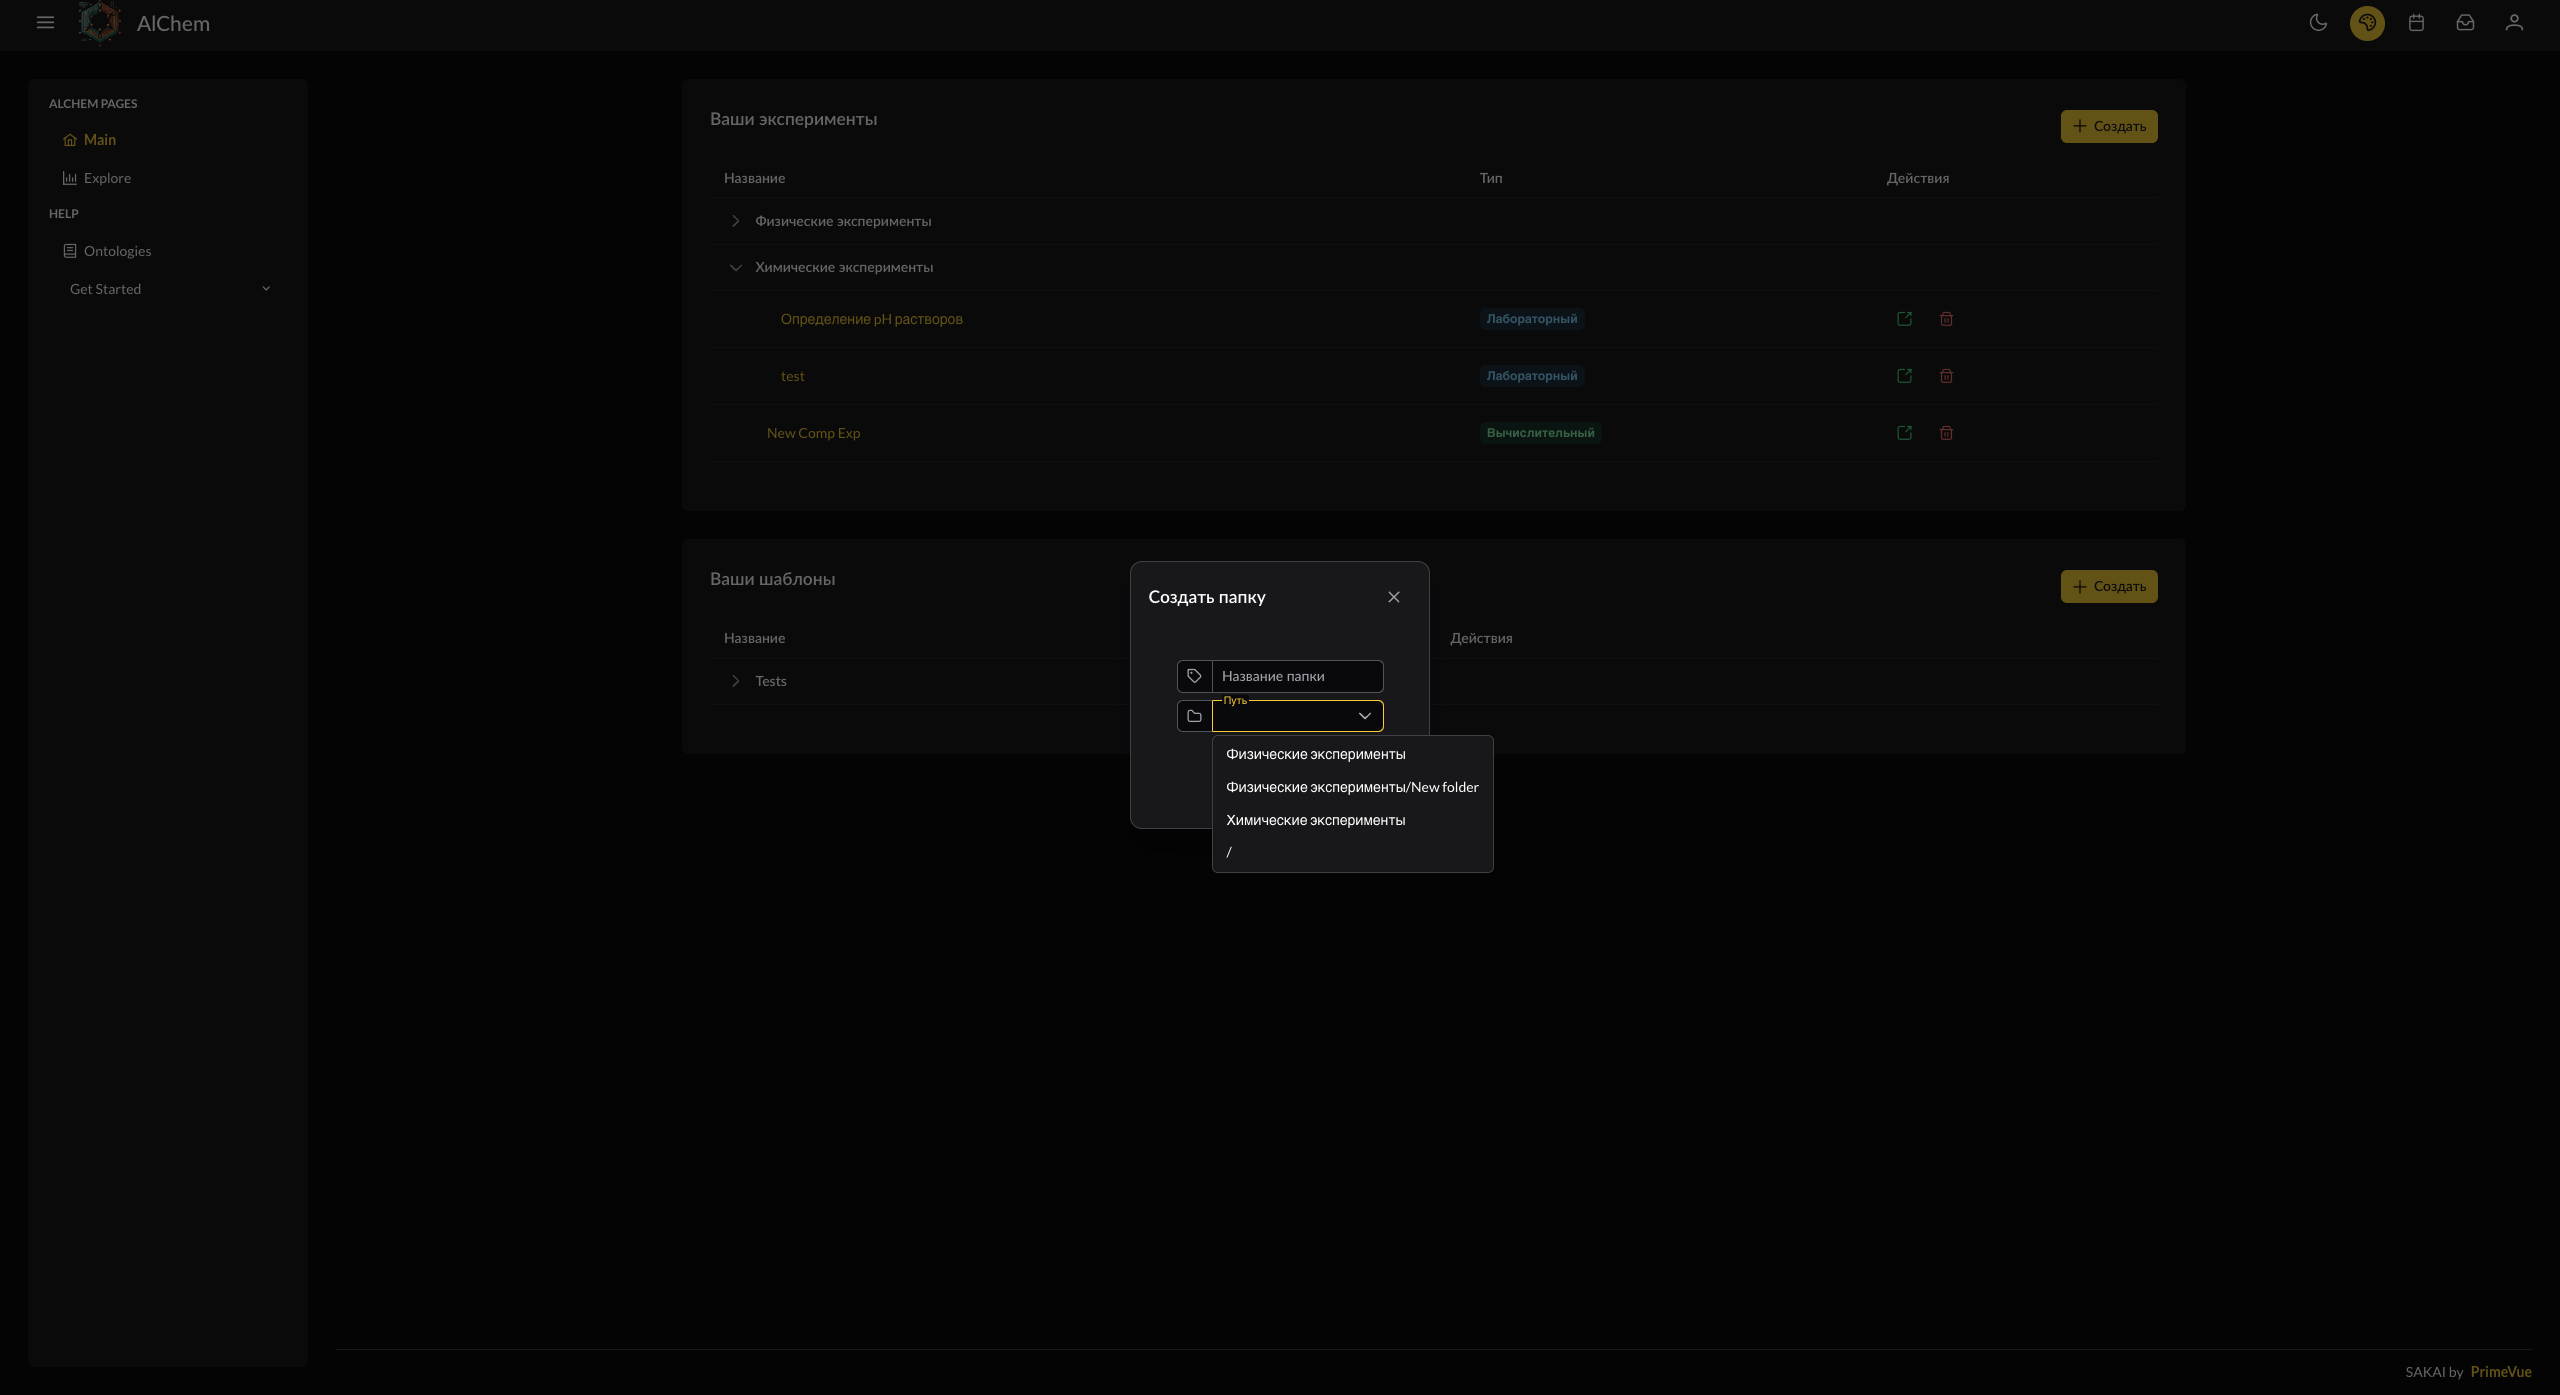
\includegraphics[width=\textwidth]{RO/img/create_folder.png} % Замените на правильный путь к изображению
    \caption{Экран: Создание папки}
    \label{fig:create_folder}
\end{figure}

\subsubsection{Экран: Ввод данных лабораторного эксперимента}
\textbf{Данные для ввода:}  
Для ввода данных в эксперимент:
\begin{enumerate}
    \item Введите описание эксперимента и данные для каждого столбца таблицы.
    \item Нажмите "Добавить строку", чтобы добавить новые данные для эксперимента или "+", чтобы добавить новый столбец.
    \item Опишите каждый столбец с помощью специального диалога
\end{enumerate}
\begin{figure}[H]
    \centering
    \begin{minipage}{0.45\linewidth}
        \centering
        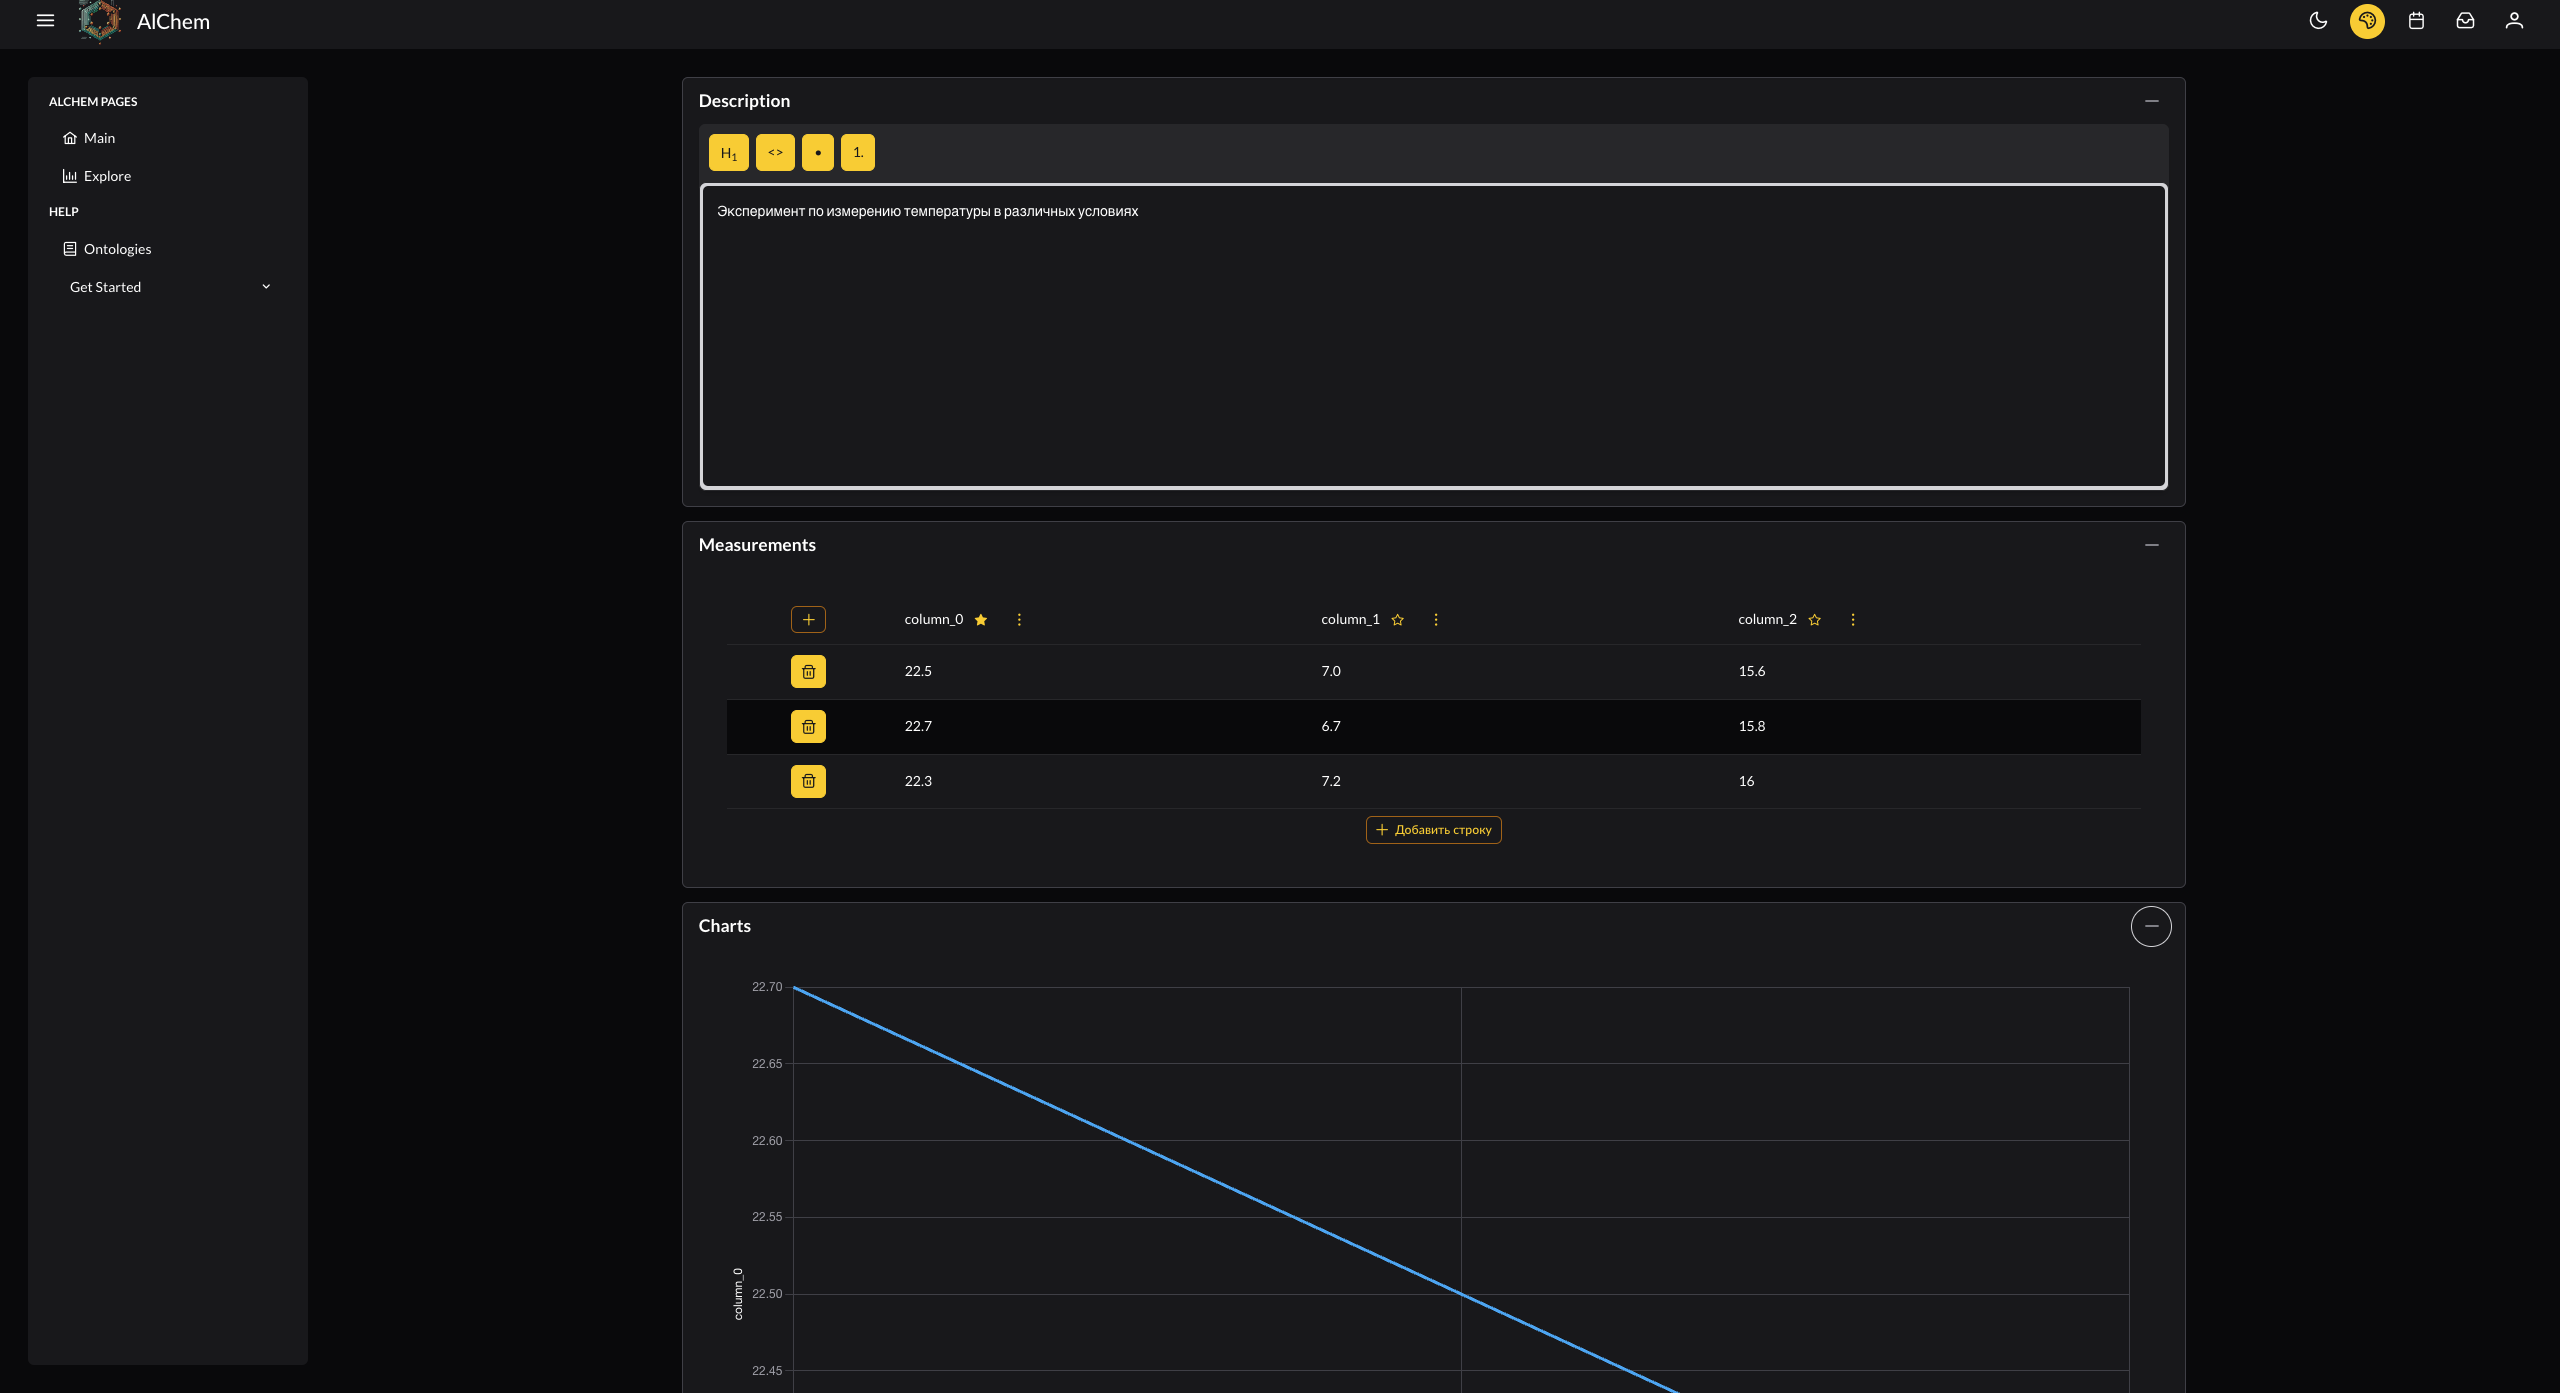
\includegraphics[width=\linewidth]{RO/img/lab_common.png}
        \caption{Экран: Ввод данных лабораторного эксперимента}
        \label{pic:mobile_version}
    \end{minipage}\hfill
    \begin{minipage}{0.45\linewidth}
        \centering
        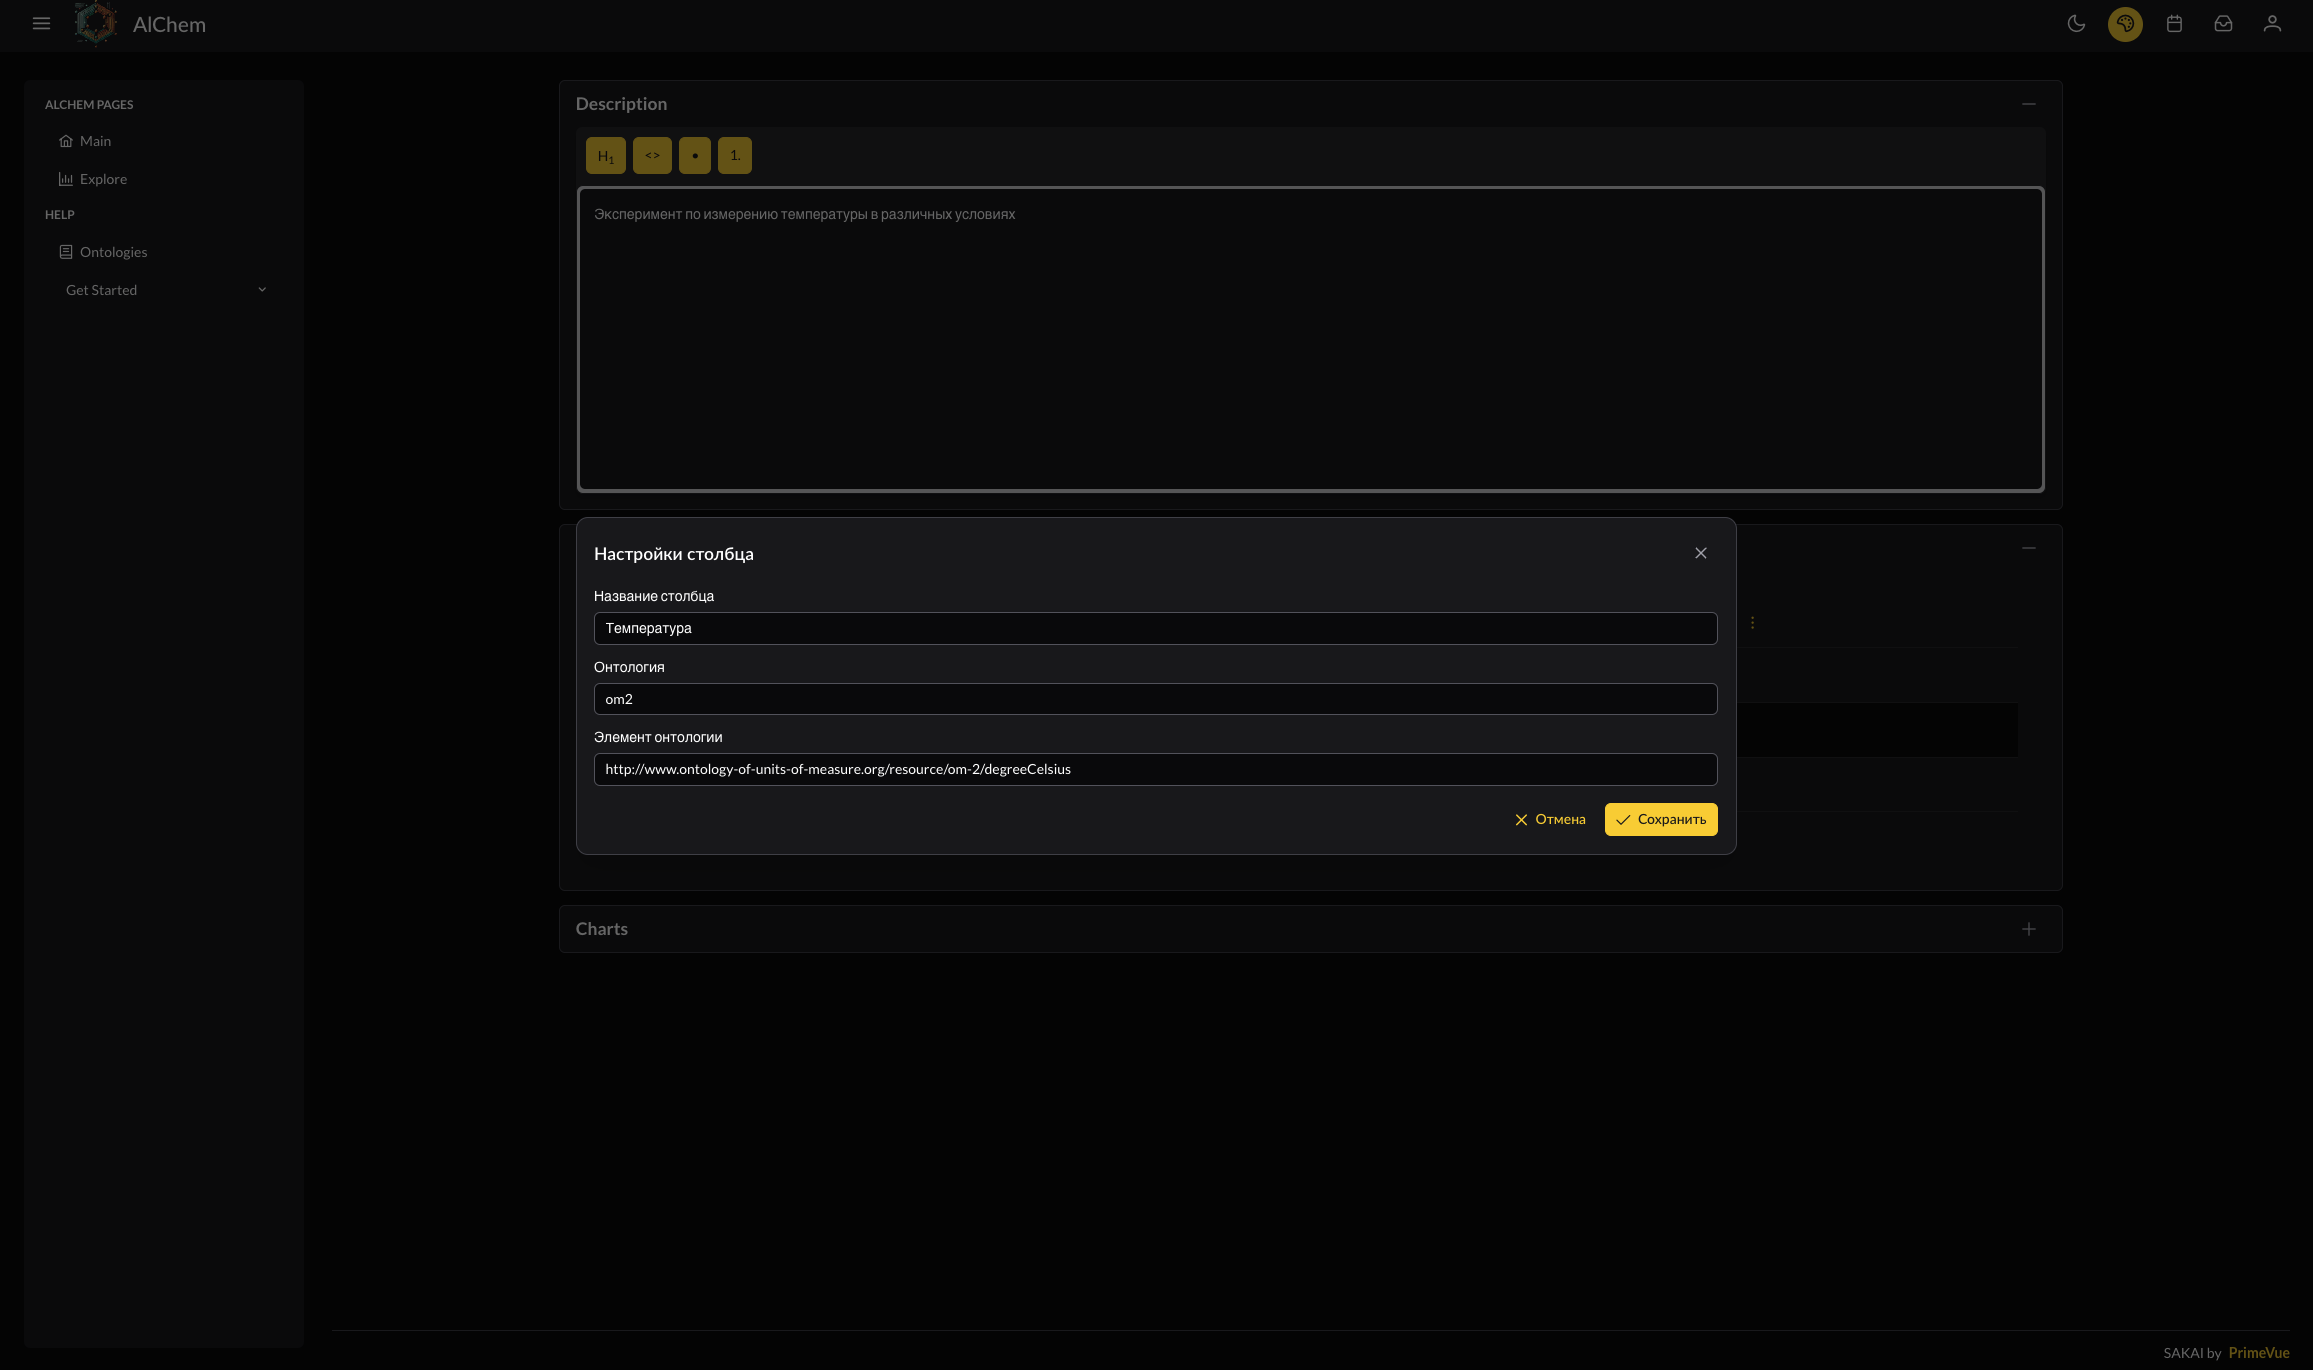
\includegraphics[width=\linewidth]{RO/img/change_column.png}
        \caption{Диалог: Настройка столбца}
        \label{pic:other_colors}
    \end{minipage}
\end{figure}

\subsubsection{Экран: Панель управления}
На этом экране отображаются все ваши эксперименты и шаблоны. Для того чтобы взаимодействовать с компонентами на этом экране:
\begin{enumerate}
    \item Просматривайте список экспериментов по категориям.
    \item Нажимайте кнопку "Создать", чтобы создать новый эксперимент или шаблон.
    \item Выполняйте действия с экспериментами, такие как перемещение или удаление, используя доступные иконки действий.
\end{enumerate}
\begin{figure}[H]
    \centering
    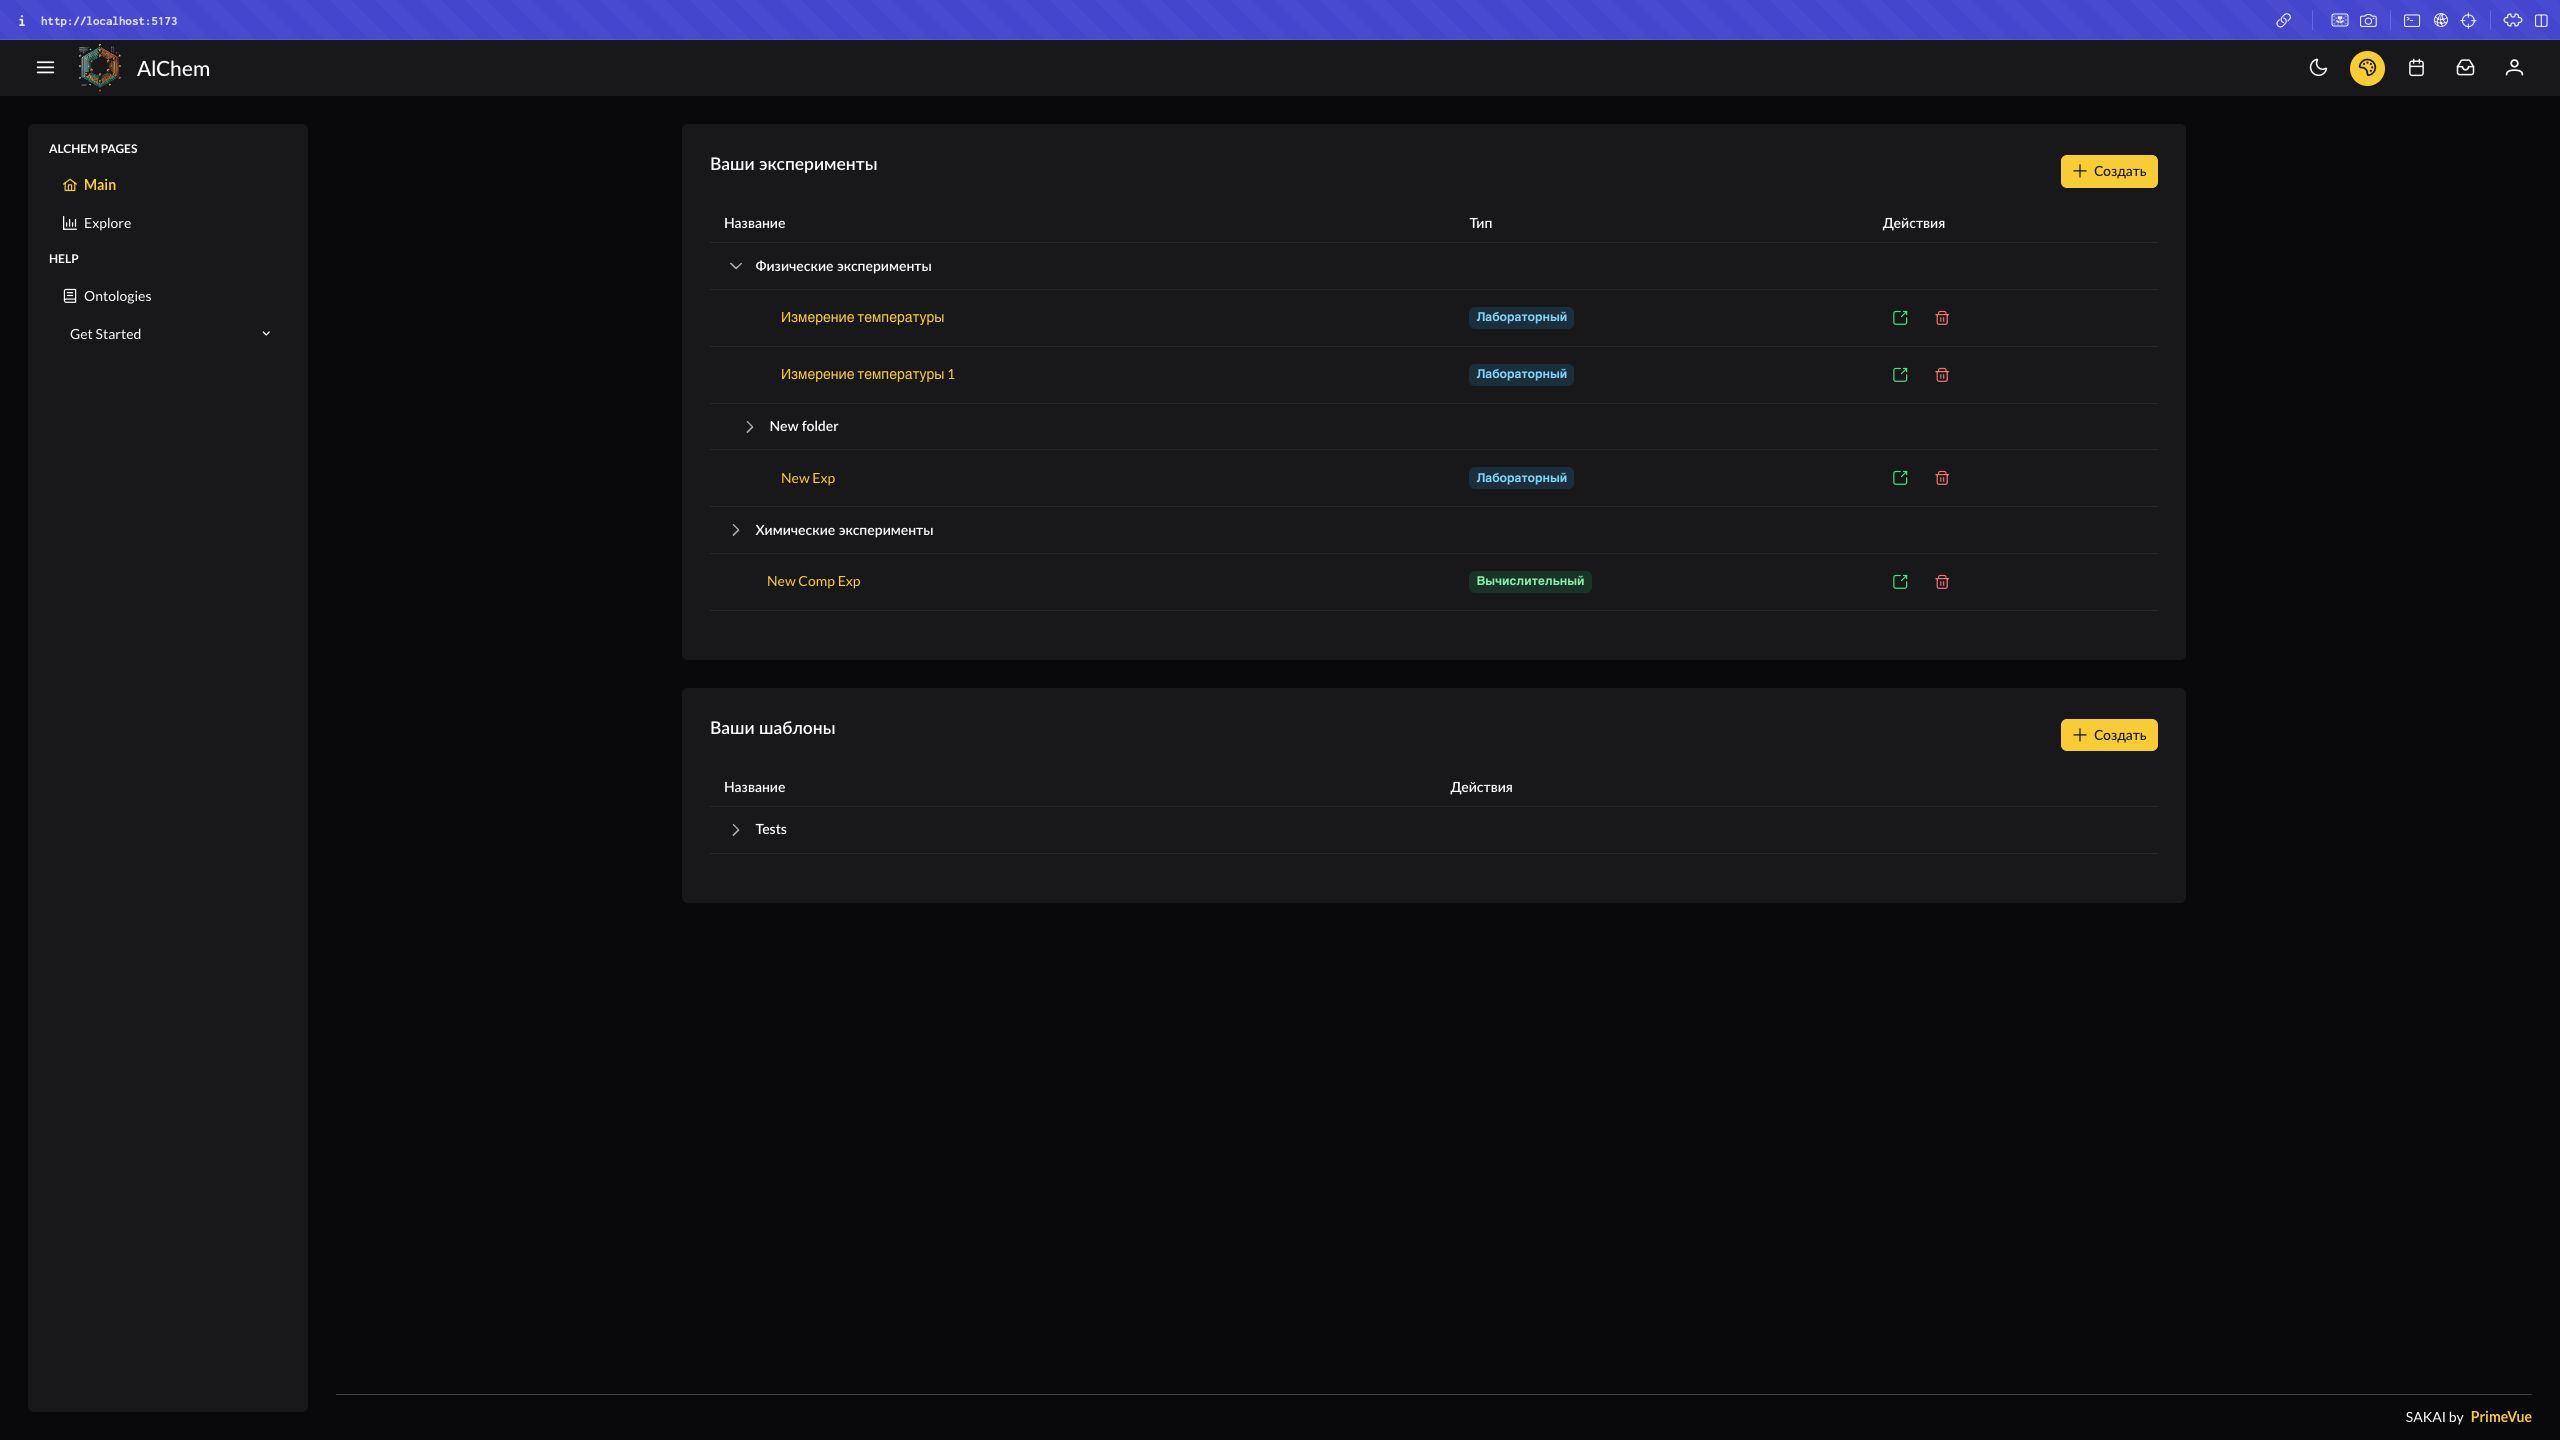
\includegraphics[width=\textwidth]{RO/img/dashboard.png} % Замените на правильный путь к изображению
    \caption{Экран: Панель управления}
    \label{fig:dashboard}
\end{figure}

\subsubsection{Экран: Перемещение эксперимента или шаблона}
Для перемещения эксперимента или шаблона между папками:
\begin{enumerate}
    \item Выберите элемент, который хотите переместить.
    \item Откроется диалоговое окно, в котором нужно выбрать новую папку.
    \item Нажмите кнопку "Переместить" для завершения операции.
\end{enumerate}
\begin{figure}[H]
    \centering
    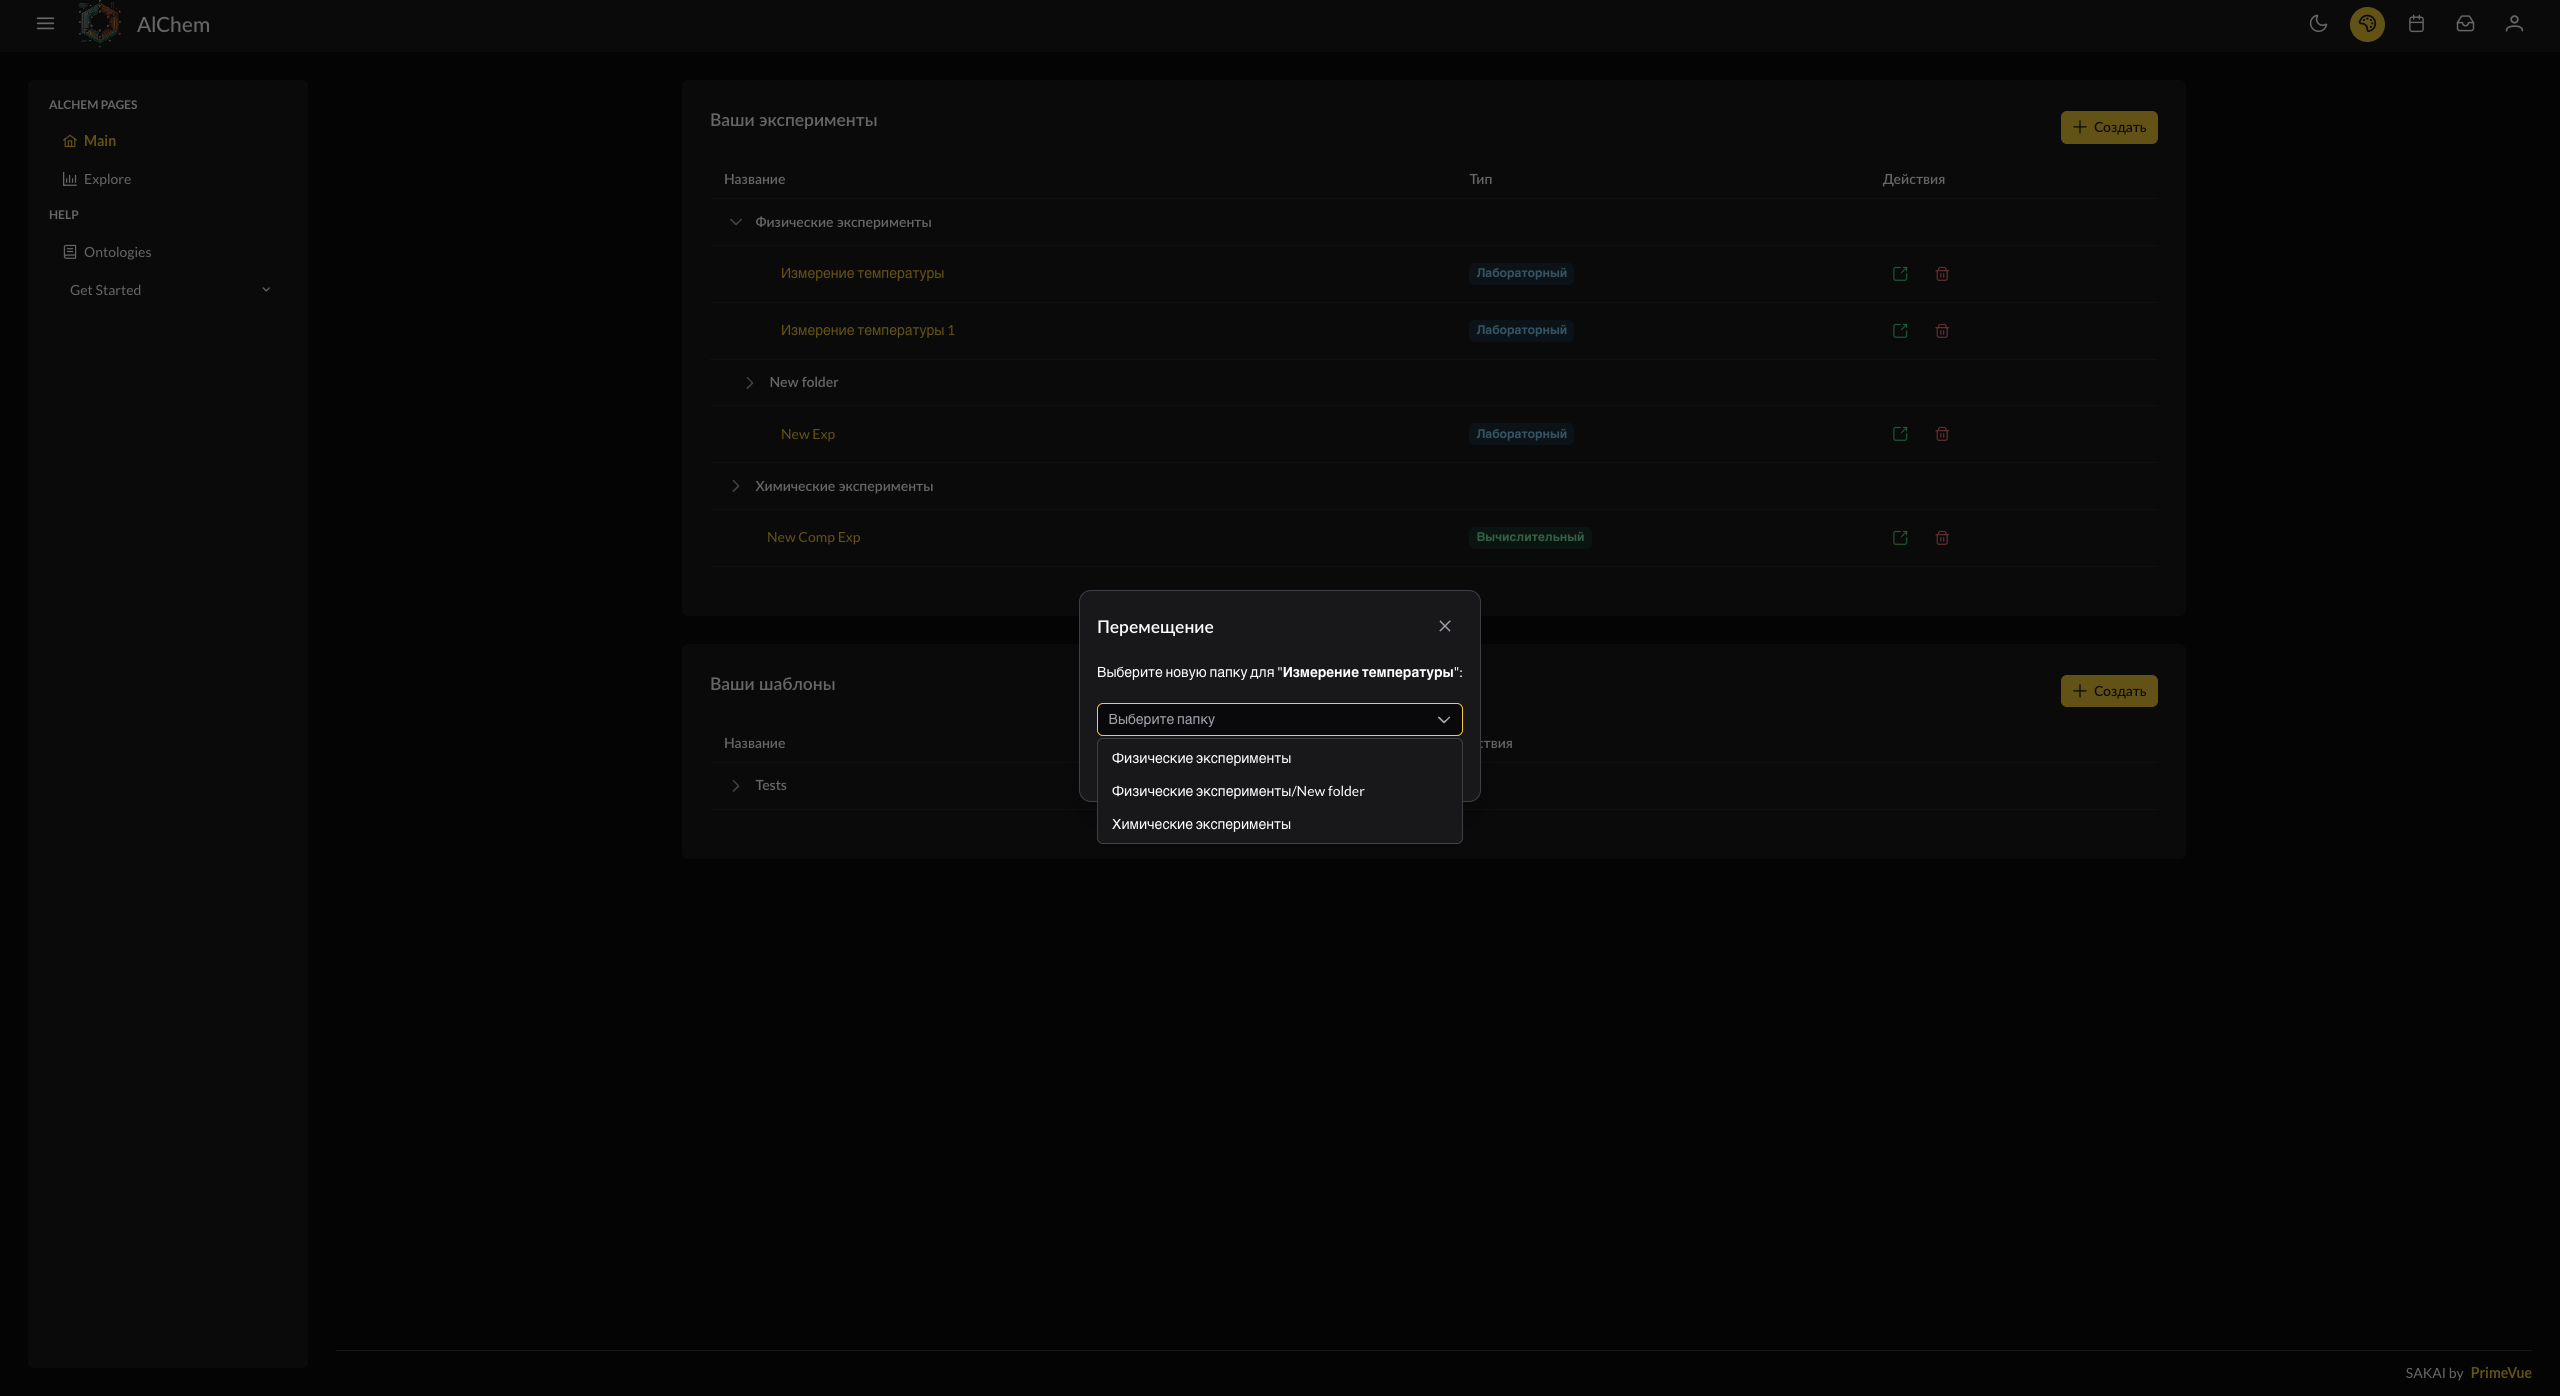
\includegraphics[width=\textwidth]{RO/img/move_dialog.png} % Замените на правильный путь к изображению
    \caption{Экран: Перемещение эксперимента или шаблона}
    \label{fig:move_dialog}
\end{figure}

\subsubsection{Экран: Вход в систему}
Для входа в систему:
\begin{enumerate}
    \item Введите ваше имя пользователя в поле "Username".
    \item Введите пароль в поле "Password".
    \item Нажмите кнопку "Sign In" для выполнения входа в систему.
\end{enumerate}
\begin{figure}[H]
    \centering
    
\includegraphics[width=\textwidth]{RO/img/signin.png} % Замените на правильный путь к изображению
    \caption{Экран: Вход в систему}
    \label{fig:signin}
\end{figure}

\subsubsection{Экран: Регистрация}
\textbf{Данные для ввода:}  
Для регистрации нового пользователя:
\begin{enumerate}
    \item Введите имя пользователя в поле "Username".
    \item Введите пароль в поле "Password".
    \item Подтвердите пароль в поле "Confirm password".
    \item Нажмите кнопку "Sign Up" для завершения регистрации.
\end{enumerate}
\begin{figure}[H]
    \centering
    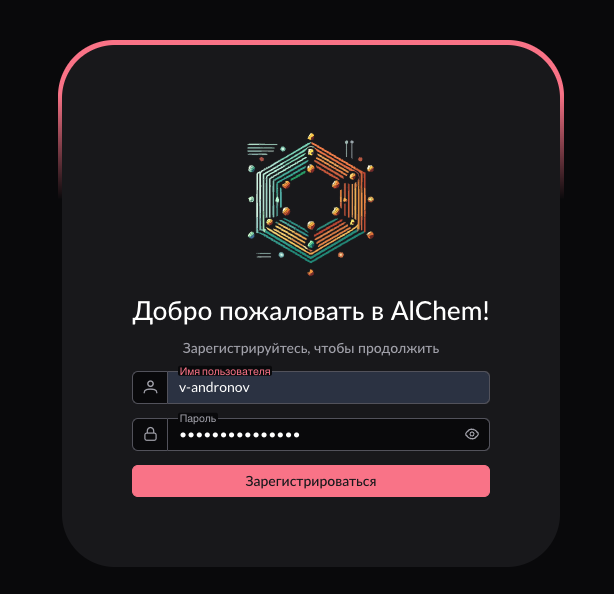
\includegraphics[width=\textwidth]{RO/img/signup.png} % Замените на правильный путь к изображению
    \caption{Экран: Регистрация}
    \label{fig:signup}
\end{figure}

\subsubsection{Экран: Ввод данных вычислительного эксперимента}
\textbf{Данные для ввода:}  
Для создания графика сравнения двух экспериментов:
\begin{enumerate}
    \item Введите описание эксперимента и данные для каждого столбца таблицы. 
    \item Каждая ячейка каждого столбца должна соответствовать формату соответствующего шаблона.
    \item Нажмите "Добавить строку", чтобы добавить новые данные для эксперимента или "+", чтобы добавить новый столбец.
\end{enumerate}
\begin{figure}[H]
    \centering
    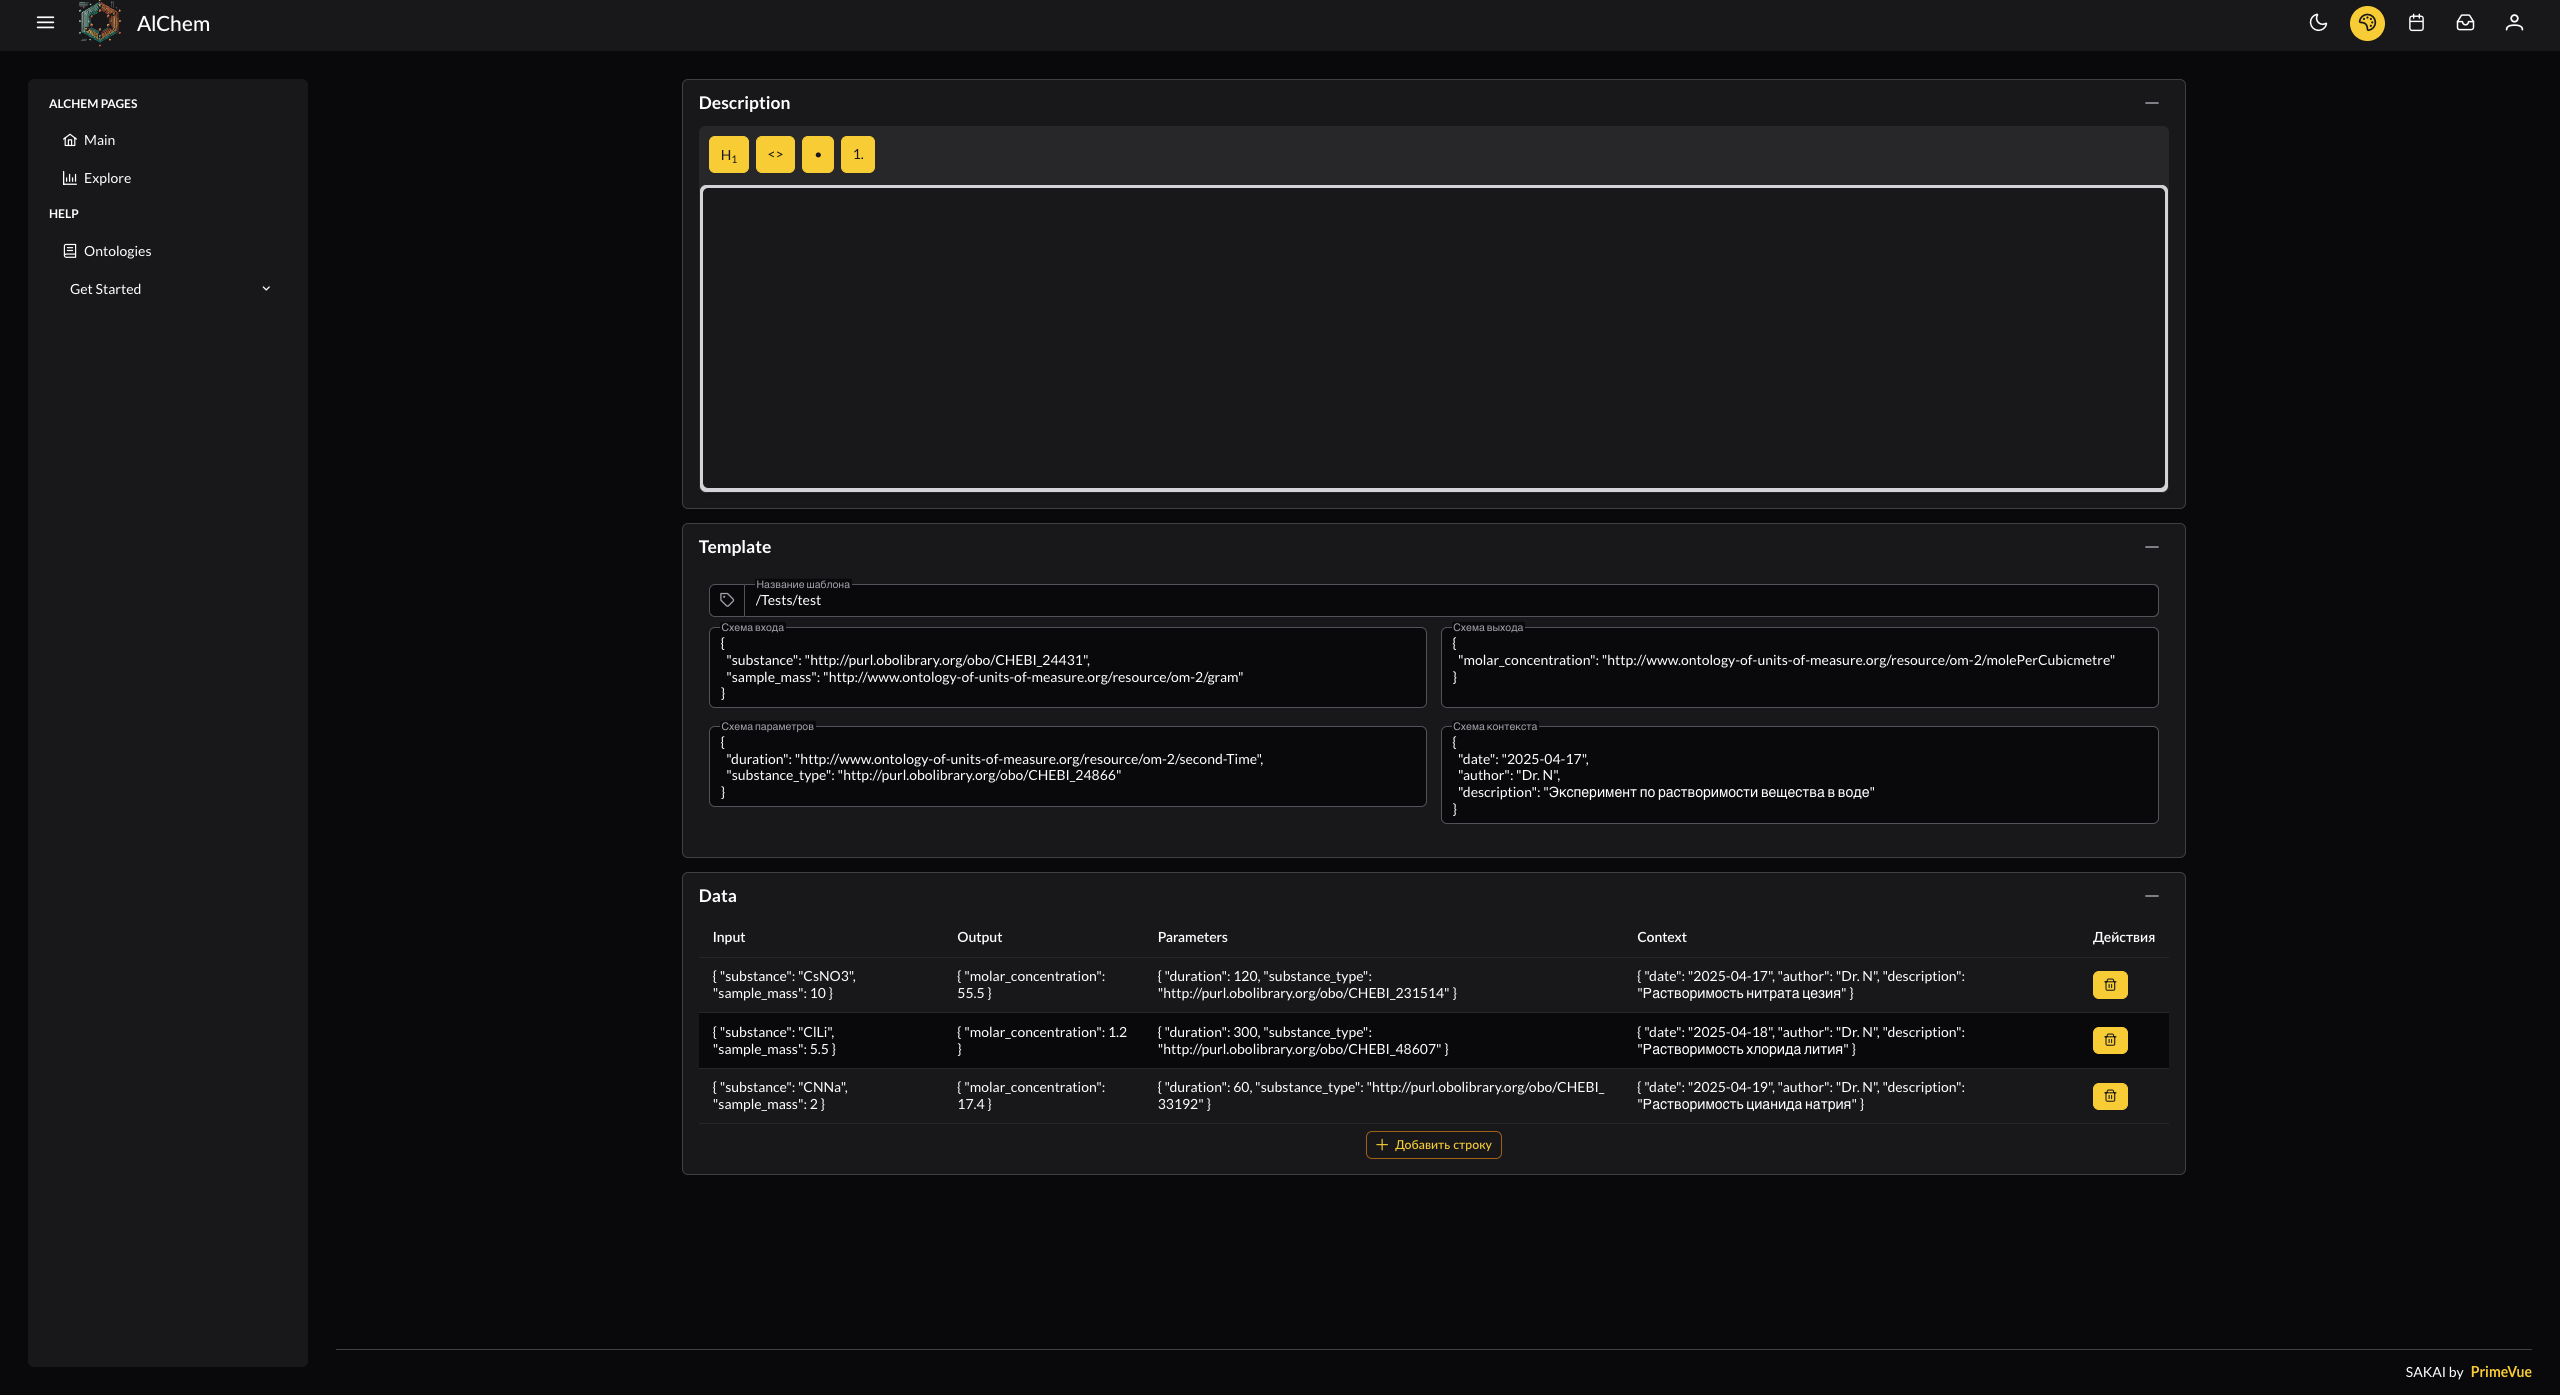
\includegraphics[width=\textwidth]{RO/img/comp_exp.png} % Замените на правильный путь к изображению
    \caption{Экран: Сравнение экспериментов}
    \label{fig:comp_exp}
\end{figure}

\subsubsection{Экран: Графики измерений}
Для отображения графиков измерений:
\begin{enumerate}
    \item Выберите один столбец главным, нажав на иконку-звёздочку рядом с его названием, все остальные будут считаться не главными (параметрами).
    \item График будет отображать изменения значений для выбранных параметров.
\end{enumerate}
\begin{figure}[H]
    \centering
    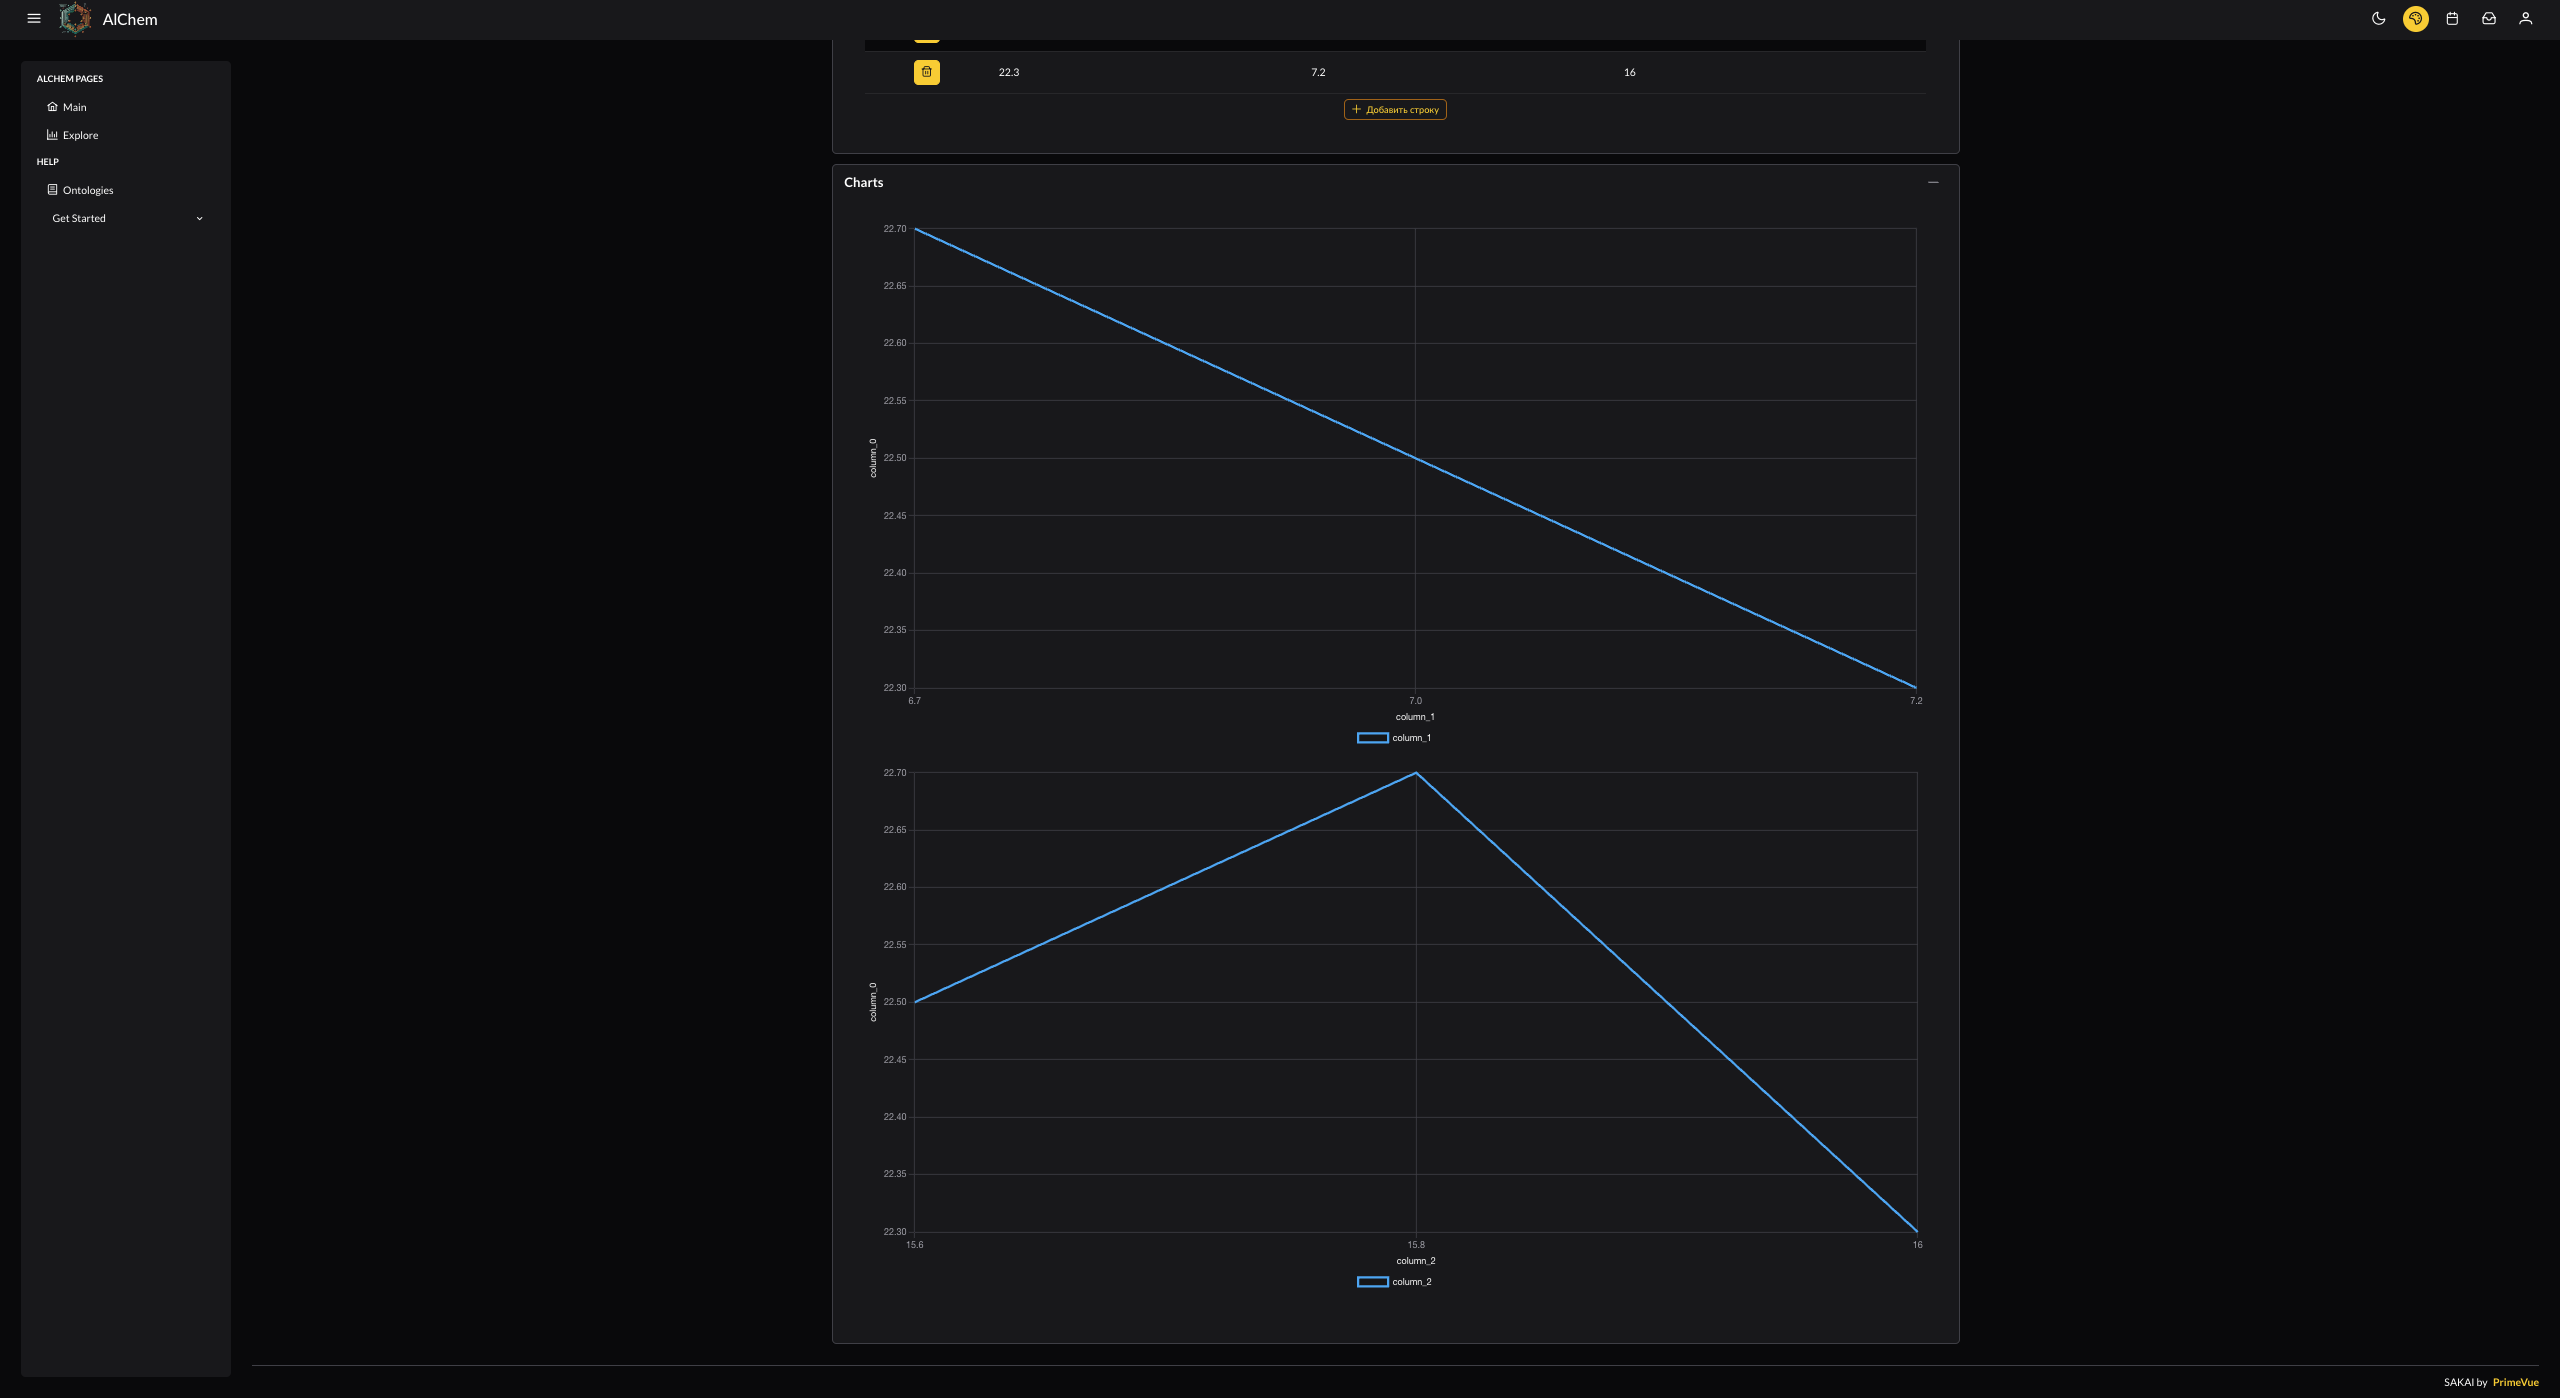
\includegraphics[width=\textwidth]{RO/img/lab_charts.png} % Замените на правильный путь к изображению
    \caption{Экран: Графики измерений}
    \label{fig:lab_charts}
\end{figure}

\section{Сообщения оператору}
\subsection{Ошибки}
\begin{itemize}
    \item Некорректный логин или пароль при аутентификации.
    \item Ошибка в формате данных при импорте.
    \item Ошибка при создании нового эксперимента.
    \item Ошибка загрузки экспериментальных данных.
    \item Ошибка обновления данных эксперимента.
    \item Не удалось сохранить изменения.
\end{itemize}

\subsection{Уведомления}
\begin{itemize}
    \item Изменения сохранены успешно.
    \item Ошибка при удалении столбца из таблицы.
    \item Ошибка при добавлении нового столбца.
\end{itemize}


\printbibliography[title=Список источников, heading=bibintoc]

\newpage
\addition{Используемые понятия и определения}{additionterms}
\phantomsection
\addcontentsline{toc}{section}{Основные определения, термины и сокращения}

\begin{description}[style=unboxed,leftmargin=0cm]

    \item[\textbf{Валидность}] -- степень соответствия полученных данных реальности.

    \item[\textbf{Вычислительный эксперимент}] -- метод исследования, при котором математические модели и компьютерные расчёты используются для анализа сложных систем и прогнозирования их поведения.

    \item[\textbf{Домен (предметная область)}] -- область знаний, к которой относится конкретное программное обеспечение.

    \item[\textbf{Интероперабельность}] -- возможность обмена и понимания данных между разными системами на основе их смыслового значения.

    \item[\textbf{Клиент-серверная архитектура}] -- принцип проектирования ПО, согласно которому клиент запрашивает данные у сервера, который их обрабатывает и отправляет обратно.

    \item[\textbf{Лабораторный эксперимент}] -- метод научного исследования, проводимый в контролируемых условиях лаборатории для проверки гипотез, изучения свойств объектов или выявления закономерностей.

    \item[\textbf{Онтология}] -- формализованное представление знаний в определённой предметной области, включающее определения понятий, их свойства и взаимосвязи между ними. Используется в искусственном интеллекте, базах знаний и прочих областях.

    \item[\textbf{Слоистая архитектура}] -- принцип проектирования ПО, согласно которому система разделена на слои, каждый из которых выполняет свою роль.

    \item[\textbf{СУБД (Система управления базами данных)}] -- программное обеспечение для создания, управления и работы с базами данных.

    \item[\textbf{API (Application Programming Interface)}] -- интерфейс программирования приложений, набор правил и инструментов для взаимодействия между программными компонентами.

    \item[\textbf{ELN (Electronic Laboratory Notebook)}] -- электронный лабораторный журнал, который используется для ведения, хранения и управления научными записями, заменяя традиционные бумажные записи.

    \item[\textbf{JWT (JSON Web Token)}] -- компактный и безопасный способ передачи информации между сторонами в виде JSON-объекта, часто используется для аутентификации.

    \item[\textbf{ORM (Object-Relational Mapping)}] -- технология, позволяющая работать с базами данных с использованием объектно-ориентированных подходов вместо SQL-запросов.

    \item[\textbf{SPA (Single Page Application)}] -- веб-приложение, которое загружается один раз и обновляет контент без полной перезагрузки страницы, улучшая пользовательский опыт.

\end{description}

\newpage
\listRegistration

\end{document}